%!TEX root = ../../csuthesis_main.tex
\chapter{最优化基本理论概述}
\section{一阶最优性条件}
\subsection{无约束优化}
\cite{王宜举2016非线性最优化理论与方法}下面是对于无约束凸优化问题的一阶最优性条件,对于其他有约束优化问题,或者将其转化为无约束问题,或者使用无约束问题近似求解(参考自课本与西瓜书)。s

\textbf{定理1} 对无约束优化问题(1.6.1), 若目标函数 $f$ 是连续可微的凸函数, 则 $x^{*}$ 为 (全局)最优解的充分必要条件是 $\nabla f\left(x^{*}\right)=\mathbf{0}$。

证明 若 $x^{*}$ 是无约束优化问题 $(1.6 .1)$ 的 (全局)最优解, 显然有 $\nabla f\left(x^{*}\right)=\mathbf{0}$. 反过来, 若 $x^{*}$ 是稳定点, 利用凸函数的性质, 对任意的 $x \in \mathbb{R}^{n}$,
$$
f(x)-f\left(x^{*}\right) \geqslant\left\langle\nabla f\left(x^{*}\right), x-x^{*}\right\rangle=0
$$

故$x^{*}$是局部最优解,又由于凸函数的性质:“凸函数是单峰函数,局部最优即为全局最优”,$x^{*}$又是全局最优解。
\subsection{带约束优化($KKT$条件)}
在机器学习模型支持向量机(Support Vector Machine)和最大熵模型(Maximum Entropy Model)中,需要用到$KKT$条件来作为理论支持,$Karush-Kuhn-Tucker (KKT)$条件是非线性规划(nonlinear programming)最佳解的必要条件。$KKT$条件将Lagrange乘数法(Lagrange multipliers)所处理涉及等式的约束优化问题推广至不等式。在实际应用上,$KKT$条件(方程组)一般不存在代数解,但将问题简化后我们可以认为符合$KKT$条件。我们在解释$KKT$条件前先引入拉格朗日乘子法。

拉格朗日乘子法(Lagrange multipliers)是一种寻找多元函数在一组约束下的极值的方法. 通过引入拉格朗日乘子, 可将有 $d$ 个变量与 $k$ 个约束条件的最 优化问题转化为具有 $d+k$ 个变量的无约束优化问题求解。

先考虑一个等式约束的优化问题. 假定 $\boldsymbol{x}$ 为 $d$ 维向量, 欲寻找 $\boldsymbol{x}$ 的某个取 值 $\boldsymbol{x}^{*}$, 使目标函数 $f(\boldsymbol{x})$ 最小且同时满足 $g(\boldsymbol{x})=0$ 的约束. 从几何角度看, 该问 题的目标是在由方程 $g(\boldsymbol{x})=0$ 确定的 $d-1$ 维曲面上寻找能使目标函数 $f(\boldsymbol{x})$ 最小化的点. 此时不难得到如下结论:

$\bullet$对于约束曲面上的任意点 $\boldsymbol{x}$, 该点的梯度 $\nabla g(\boldsymbol{x})$ 正交于约束曲面;

$\bullet$在最优点 $\boldsymbol{x}^{*}$, 目标函数在该点的梯度 $\nabla f\left(\boldsymbol{x}^{*}\right)$ 正交于约束曲面.

由此可知, 在最优点 $\boldsymbol{x}^{*}$, 如附图B.1 所示, 梯度 $\nabla g(\boldsymbol{x})$ 和 $\nabla f(\boldsymbol{x})$ 的方向必相同 或相反, 即存在 $\lambda \neq 0$ 使得
$$
\nabla f\left(x^{*}\right)+\lambda \nabla g\left(x^{*}\right)=0
$$

$\lambda$ 称为拉格朗日乘子. 定义拉格朗日函数
$$
L(\boldsymbol{x}, \lambda)=f(\boldsymbol{x})+\lambda g(\boldsymbol{x})
$$

不难发现, 将其对 $\boldsymbol{x}$ 的偏导数 $\nabla_{x} L(\boldsymbol{x}, \lambda)$ 置零即得第一个式子, 同时, 将其对 $\lambda$ 的 偏导数 $\nabla_{\lambda} L(\boldsymbol{x}, \lambda)$ 置零即得约束条件 $g(\boldsymbol{x})=0$. 于是, 原约束优化问题可转化 为对拉格朗日函数 $L(\boldsymbol{x}, \lambda)$ 的无约束优化问题。
\begin{figure}[hbt]
    \centering
    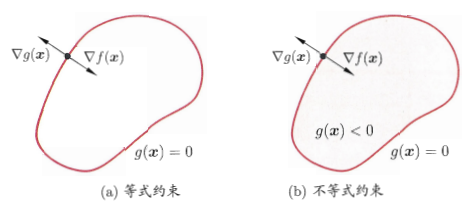
\includegraphics[width=0.7\linewidth]{KKT.png}
    \caption{KKT条件}
    \label{KKT}
\end{figure}

现在考虑不等式约束 $g(x) \leqslant 0$, 如图\ref{KKT}所示, 此时最优点 $x^{*}$ 或在 $g(\boldsymbol{x})<0$ 的区域中, 或在边界 $g(\boldsymbol{x})=0$ 上. 对于 $g(\boldsymbol{x})<0$ 的情形, 约本 $g(x) \leqslant 0$ 不起作用,可直接通过条件: $\nabla f(x)=0$ 來获得最优点; 这等价于将 $\lambda$ 置零然后对$\nabla_{x}L(x,\lambda)$置零得到最优点。$g(x)=0$的情形类似于上面等式约束的分析,但需注意的是, 此时 $\nabla f\left(x^{*}\right)$ 的方向必与 $\nabla g\left(x^{*}\right)$相反,即存在常数 $\lambda>0$ 使得 $\nabla f\left(\boldsymbol{x}^{*}\right)+\lambda \nabla g\left(\boldsymbol{x}^{*}\right)=0$。 整合这两种情形, 必满足 $\lambda g(\boldsymbol{x})=0$。因此,在约束 $g(\boldsymbol{x}) \leqslant 0$ 下最小化 $f(\boldsymbol{x})$, 可转化为在如下约束下最小化拉格朗日函数:
$$
\left\{\begin{array}{l}
g(\boldsymbol{x}) \leqslant 0 \\
\lambda \geqslant 0 \\
\mu_{j} g_{j}(\boldsymbol{x})=0
\end{array}\right.
$$

上式称为 Karush-Kuhn-Tucker (简称KKT)条件.

上述做法可推广到多个约束. 考虫具有 $m$ 个等式约束和 $n$ 个不等式约束, 且可行域 $\mathbb{D} \subset \mathbb{R}^{d}$ 非空的优化问题
$$
\begin{array}{lll}
\min _{\boldsymbol{x}} & f(\boldsymbol{x}) & \\
\text { s.t. } & h_{i}(\boldsymbol{x})=0 & (i=1, \ldots, m) \\
& g_{j}(\boldsymbol{x}) \leqslant 0 \quad(j=1, \ldots, n)
\end{array}
$$

引入拉格朗日乘子 $\boldsymbol{\lambda}=\left(\lambda_{1}, \lambda_{2}, \ldots, \lambda_{m}\right)^{\mathrm{T}}$ 和 $\boldsymbol{\mu}=\left(\mu_{1}, \mu_{2}, \ldots, \mu_{n}\right)^{\mathrm{T}}$, 相应的拉格朗日函数为
$$
L(\boldsymbol{x}, \boldsymbol{\lambda}, \boldsymbol{\mu})=f(\boldsymbol{x})+\sum_{i=1}^{m} \lambda_{i} h_{i}(\boldsymbol{x})+\sum_{j=1}^{n} \mu_{j} g_{j}(\boldsymbol{x})
$$

由不等式约束引入的 KKT 条件 $(j=1,2, \ldots, n)$ 为
$$
\left\{\begin{array}{l}
g_{j}(\boldsymbol{x}) \leqslant 0 \\
\mu_{j} \geqslant 0 \\
\mu_{j} g_{j}(\boldsymbol{x})=0
\end{array}\right.
$$

\section{二阶最优性条件}
目标函数梯度为0的点被称为问题的稳定点,但是稳定点不一定是最优解,还可能是最大值解。所以要确认一个解是不是最优解,还需要考察目标函数在该点的二阶最优性条件。

\subsection{无约束优化}
\textbf{定理2.1} (二阶必要条件) 设 $x^{*} \in \mathbb{R}^{n}$ 是无约束优化问题 (1.6.1) 的局部最优解, 且 $f(x)$ 在 $x^{\star}$ 点附近二阶连续可微. 则 $\nabla f\left(x^{*}\right)=0, \nabla^{2} f\left(x^{\star}\right)$ 半正定。

证明 由定理1.6.1知 $\nabla f\left(x^{*}\right)=0$. 若 $\nabla^{2} f\left(x^{\star}\right)$ 非半正定, 则存在单位向量 $\boldsymbol{d} \epsilon$ $\mathbb{R}^{n}$, 使 $\boldsymbol{d}^{\mathrm{T}} \nabla^{2} f\left(\boldsymbol{x}^{*}\right) \boldsymbol{d}<0$. 对 $\alpha>0$ 充分小, 利用Taylor展式,

$f\left(\boldsymbol{x}^{*}+\alpha \boldsymbol{d}\right)=f\left(\boldsymbol{x}^{*}\right)+\alpha \nabla f\left(\boldsymbol{x}^{*}\right)^{\mathrm{T}} \boldsymbol{d}+\frac{1}{2} \alpha^{2} \boldsymbol{d}^{\mathrm{T}} \nabla^{2} f\left(\boldsymbol{x}^{*}\right) \boldsymbol{d}+o\left(\alpha^{2}\right)<f\left(\boldsymbol{x}^{*}\right)$,

这与 $x^{*}$ 是局部最优解矛盾. 结论得证。

上述结论给出的最优性条件不是充分的. 如单元函数 $f(x)=x^{3}$ 在 $x=0$ 点同 时满足一阶和二阶最优性必要条件, 但它并不是该函数的局部最优值点。

\textbf{定理2.2} (二阶充分条件) 设 $x^{*} \in \mathbb{R}^{n}$ 满足 $\nabla f\left(x^{*}\right)=0$ 且 $\nabla^{2} f\left(x^{*}\right)$ 正定, 则 $x^{*}$ 是无约束优化问题(1.6.1)的严格局部最优解。

证明 对任意充分靠近 $x^{*}$ 的 $x \in \mathbb{R}^{n}$, 存在单位向量 $d \in \mathbb{R}^{n}$ 及充分小的 $\alpha>$ 0 使 $\boldsymbol{x}=\boldsymbol{x}^{*}+\alpha \boldsymbol{d}$. 由 Taylor展式及 $\nabla^{2} f\left(\boldsymbol{x}^{*}\right)$ 的正定性得
$$
f(x)=f\left(x^{*}\right)+\frac{1}{2} \alpha^{2} d^{\mathrm{T}} \nabla^{2} f\left(x^{*}\right) d+o\left(\alpha^{2}\right)>f\left(x^{*}\right)
$$

从而, $x$ * 是 (1.6.1) 的严格局部最优解。

同样,上述结论给出的二阶充分性条件也不是必要的. 如零点是单元函数 $f(x)$ $=x^{4}$ 的严格局部最优解, 但上述二阶充分性条件在该点并不成立. 由此推断,无约 束优化问题不存在充分必要的最优性条件。

无约束优化问题的二阶最优性条件是借助目标函数在局部最优值点邻域上 的凸性来刻画.一般的优化方法只能保证迭代点列的极限点满足一阶必要条件, 而不能保证满足二阶充分条件. 换句话讲, 这些方法只能得到稳定点, 只有在特殊 情况下,才能保证问题的稳定点为其全局最优解。
\subsection{带约束优化}
约束优化问题的最优值点末必满足 KKT 条件, 而 K-T 点也末必是最优值点. 那么, 在什么情况下, 约束优化问题的 $\mathrm{K}-\mathrm{T}$ 点为最优值点呢?

考虑如下约束优化问题
$$
\begin{array}{cl}
\min & f(\boldsymbol{x})=x_{1}^{2}+x_{2}^{2} \\
\text { s.t. } & x_{1}^{2}+x_{2}-1 \geqslant 0 .
\end{array}
$$

容易验证 $x^{*}=(0,1)^{\mathrm{T}}$ 是其 $\mathrm{K}-\mathrm{T}$ 点, 并且 $\nabla^{2} f(x)$ 在 $x^{*}$ 点正定. 但 $x^{*}$ 并非该问 题的局部最优值点. 事实上, 约束区域的边界点 $\left(x_{1}, 1-x_{1}^{2}\right)^{\mathrm{T}}$ 对应的目标函数值为 $1-x_{1}^{2}+x_{1}^{4}$. 只要 $x_{1} \in(0,1)$, 就有 $f(x)<f\left(x^{*}\right)$.

该例子说明, 尽管目标函数在 K-T 点 $x^{*}$ 的 Hesse 阵正定, 但 $x^{*}$ 末必是该问 题的局部最优解, 原因很简单, 因为 $x^{*}$ 不是目标函数的稳定点. 与无约束优化问 题的二阶最优性条件不同, 约束优化问题的二阶最优性条件是建立在 Lagrange 函 数关于 $x$ 的 Hesse 阵在最优值点的临界锥上的半正定性上.

\textbf{定理2.3}(二阶必要条件) 设 $x^{*}$ 是约束优化问题
$$
\min \left\{f(\boldsymbol{x}) \mid c_{i}(\boldsymbol{x})=0, i \in \mathcal{E} ; c_{i}(\boldsymbol{x}) \geqslant 0, i \in \mathcal{I}\right\}
$$

的局部最优解, $\left(x^{*}, \lambda^{*}\right)$ 为其 $\mathrm{K}-\mathrm{T}$ 对. 若约束函数全是线性的或者 $\nabla c_{i}\left(x^{*}\right), i \in$ $\mathcal{A}\left(x^{*}\right)$ 线性无关, 则对于满足 $s^{\mathrm{T}} \nabla c_{i}\left(x^{*}\right)=0, i \in \mathcal{A}\left(x^{*}\right)$ 的任意 $s \in \mathbb{R}^{n}$ 有
$$
\boldsymbol{s}^{\mathrm{T}} \nabla_{x x} L\left(\boldsymbol{x}^{*}, \boldsymbol{\lambda}^{*}\right) \boldsymbol{s} \geqslant 0 .
$$

\textbf{定理2.4} (二阶充分条件) 设 $\left(x^{*}, \lambda^{*}\right)$ 为约束优化问题的 $\mathrm{K}-\mathrm{T}$ 对. 若对任意满足
$$
\begin{cases}s^{\mathrm{T}} \nabla c_{i}\left(x^{*}\right)=0, & \text { 若 } i \in \mathcal{E}, \\ s^{\mathrm{T}} \nabla c_{i}\left(x^{*}\right) \geqslant 0, & \text { 若 } \lambda_{i}^{*}=0, i \in \mathcal{I}\left(x^{*}\right), \\ s^{\mathrm{T}} \nabla c_{i}\left(x^{*}\right)=0, & \text { 若 } \lambda_{i}^{*}>0, i \in \mathcal{I}\left(x^{*}\right)\end{cases}
$$

的非零向量 $s \in \mathbb{R}^{n}$ 都有 $s^{\mathrm{T}} \nabla_{x x} L\left(x^{*}, \lambda^{*}\right) s>0$, 则 $x^{*}$ 是约束优化问题 (7.2.2) 的 严格局部最优解. 进一步, 存在 $\gamma>0$ 和 $\delta>0$ 使对任意的 $x \in N\left(x^{*}, \delta\right) \cap \Omega$, 成立
$$
f(x) \geqslant f\left(x^{*}\right)+\gamma\left\|x-x^{*}\right\|^{2} .
$$

优化方法大多基于上述条件判断收敛性,所以不管在理论分析上还是实际使用中上述方法都发挥很大的作用。
\chapter{最优化部分算法分析}
下面我们列举了部分最优化的算法并将其分类,如表\ref{algorithm}。然后针对表格中的无约束最优化算法分别进行分析。(启发式算法将在拓展分析部分结合实例说明)
\vspace{-0.5cm}
% Table generated by Excel2LaTeX from sheet 'Sheet1'
\begin{table}[htbp]
  \centering
  \caption{优化算法}
    \begin{tabular}{ccc}
    \toprule
    \toprule
    \multicolumn{1}{m{5em}}{一级分类} & \multicolumn{1}{m{4.51em}}{二级分类} & \multicolumn{1}{m{6.89em}}{算法} \\
    \midrule
    \multirow{11}[6]{*}{无约束优化} & \multirow{2}[2]{*}{模式搜索法} & 坐标轮换法 \\
          &       & 单纯形法 \\
\cmidrule{2-3}          & \multirow{4}[2]{*}{线搜索方法} & 最速下降法 \\
          &       & 牛顿法 \\
          &       & 共轭梯度法 \\
          &       & 拟牛顿法 \\
\cmidrule{2-3}          & \multirow{5}[2]{*}{启发式算法} & 随机算法 \\
          &       & 禁忌算法 \\
          &       & 模拟退火算法 \\
          &       & 粒子群算法 \\
          &       & 遗传算法... \\
    \midrule
    \multirow{4}[2]{*}{带约束优化} & \multirow{4}[2]{*}{} & 梯度投影方法 \\
          &       & 内点罚函数方法 \\
          &       & 外点罚函数方法 \\
          &       & 乘子罚函数方法 \\
    \bottomrule
    \bottomrule
    \end{tabular}%
  \label{algorithm}%
\end{table}%
\section{模式搜索法}
在运筹学中,单纯形法是解决线性规划问题的一个有效的算法。线性规划就是在一组线性约束条件下,求解目标函数最优解的问题,是一类经典的最优化算法。具体理论分析参见王周宏老师的运筹学基础\cite{王周宏2011运筹学基础}

\section{线搜索方法}
\cite{王宜举2016非线性最优化理论与方法}在一学期的学习中,我发现步长规则在各类算法中都有使用,所以步长规则的选取是很重要的一个方面。以线搜索方法为例,设 $d_{k}$ 为目标函数在 $x_{k}$ 点的下降方向. 为求目标函数的最小值, 一个自然的 想法是沿该方向寻求一个新点使目标函数有最大程度的下降, 也就是取步长
$$
\alpha_{k}=\arg \min _{\alpha \geqslant 0} f\left(\boldsymbol{x}_{k}+\alpha d_{k}\right) .
$$

这样的 $\alpha_{k}$ 称为精确步长, 又称最优步长。 虽然在实际中这种求解最优步长的算法在某些例子中表现不好,可能因为其最优步长的求解计算量过大,但是最优步长在理论上有很好的性质。根据最优性条件, 该步长满足如下正交性 条件:
$$
\boldsymbol{d}_{k}^{\mathrm{T}} \nabla f\left(\boldsymbol{x}_{k}+\alpha_{k} \boldsymbol{d}_{k}\right)=0 .
$$

该步长规则称为最优步长规则, 又称精确线搜索步长规则。该步长规则下的线搜索
算法模型为
\begin{table}[htbp]
  \centering
    \begin{tabular}{l}
	\bottomrule
	\bottomrule
	线搜索方法,即$V \approx v_{\pi}$ \\
    \midrule
	步 1\quad 取初始点 $x_{0} \in \mathbb{R}^{n}$ 和参数 $\varepsilon \geqslant 0$. 令 $k=0$ \\
    步 2\quad 若 $\left\|g_{k}\right\| \leqslant \varepsilon$, 算法终止; 否则, 进入下一步 \\
    步 3\quad 计算下降方向 $\boldsymbol{d}_{k}$, 使 $\boldsymbol{d}_{k}^{\mathrm{T}} g_{k}<0$ \\
    步 4\quad 计算步长 $\alpha_{k}=\arg \min \left\{f\left(x_{k}+\alpha d_{k}\right) \mid \alpha \geqslant 0\right\}$ \\
    步 5\quad 令 $\boldsymbol{x}_{k+1}=\boldsymbol{x}_{k}+\alpha_{k} \boldsymbol{d}_{k}, k=k+1$, 转步 2 \\
    \bottomrule
	\bottomrule
	\end{tabular}%
  \label{algorithm0}%
\end{table}%

在实际中,可以不取最优步长进行优化,对此也有很多种解法,称为非精确线搜索方法。典型的方法有Armijo、Wolfe、Strong Wolfe步长规则。最速下降法、牛顿法、共轭梯度法、拟牛顿法等算法都会用到这些步长规则。

\section{几类无约束优化算法框架}
接下来介绍几类学到的无约束优化算法\cite{王宜举2016非线性最优化理论与方法}。
\subsection{最速下降法}
框架如下:

			步 1 . 取初始点 $x_{0} \in \mathbb{R}^{n}$ 和参数 $\varepsilon \geqslant 0$. 令 $k=0$.

			步 2. 若 $\left\|g_{k}\right\| \leqslant \varepsilon$, 算法终止; 否则, 进入下一步.

			步 3. 计算下降方向 $\boldsymbol{d}_{k}$, 使 $\boldsymbol{d}_{k}^{\mathrm{T}} g_{k}<0$.

			步 4. 计算步长 $\alpha_{k}=\arg \min \left\{f\left(x_{k}+\alpha d_{k}\right) \mid \alpha \geqslant 0\right\}$.

			步 5. 令 $\boldsymbol{x}_{k+1}=\boldsymbol{x}_{k}+\alpha_{k} \boldsymbol{d}_{k}, k=k+1$, 转步 2 .
\subsection{牛顿法}
框架如下:

步1. 取初始点 $x_{0}$ 及精确参数 $\varepsilon \geq 0$, 令 $k=0$.

步2. 若 $\left\|g_{k}\right\| \leq \varepsilon$, 算法终止, 否则进入下一步.

步3. 令 $x_{k+1}=x_{k}-G_{k}^{-1} g_{k}, k=k+1$, 转步 2 .
\subsection{非线性共轭梯度法}
框架如下:

步1. 取初始点 $x_{0}$ 及终止参数 $\varepsilon \geq 0, d_{0}=-g_{0}$. 令 $k=0$.

步 2 . 若 $\left\|g_{k}\right\| \leq \varepsilon$, 算法终止, 否则进入下一步.

步3. 按照一定的步长规则(FR,PR,CW,Dixon规则)选取步长 $\alpha_{k 1}^{1}$ 

步4. 计算 $x_{k+1}=x_{k}+\alpha_{k} d_{k}, g_{k+1}=\nabla f\left(x_{k+1}\right)$,

\subsection{拟牛顿法}
框架如下:

步1. 取 $\boldsymbol{x}_{0} \in \mathbb{R}^{n}, n$ 阶阵 $\boldsymbol{H}_{0}$ 和参数 $\varepsilon \geqslant 0$. 令 $k=0$.

步2. 计算 $\boldsymbol{d}_{k}=-\boldsymbol{H}_{k} \boldsymbol{g}_{k}$. 令 $\boldsymbol{x}_{k+1}=\boldsymbol{x}_{k}+\alpha_{k} \boldsymbol{d}_{k}$, 其中, 步长 $\alpha_{k}$ 由线搜索产生. 若 $\left\|\boldsymbol{g}_{k+1}\right\| \leqslant \varepsilon$, 算法停止; 否则, 转下一步.

步3. 按照一定的校正公式求$H_{k+1},\ k = k + 1$,转步2. 
\subsection{Gauss-Newton算法}
框架如下:

步1. 取初始点 $x_{0}$ 及精度参数 $\varepsilon \geq 0$, 令 $k=0$.

步2. 若 $\left\|g_{k}\right\| \leq \varepsilon$, 算法终止, 否则进入下一步.

步3. 计算Gauss-Newton方向 $d_{k}=-\left(J_{k}^{T} J_{k}\right)^{-1} J_{k}{ }^{T} r_{k}$

步4. 利用线搜索步长规则选取步长 $\alpha_{k}$.

步5. 令 $x_{k+1}=x_{k}+\alpha_{k} d_{k}, k=k+1$, 转步 2 .
\subsection{信赖域方法}
这个方法的思想很重要,强化学习最著名的算法PPO就是借助这个方法建立起来的,也是因为这个算法,强化学习真正进入大众的视野,被人们广泛使用。信赖域方法基本框架如下:

步1. 取最大信赖域半径 $\hat{\Delta}$, 初始点 $x_{0}$, 参数 $\Delta_{0} \in(0, \hat{\Delta}], \eta \in\left[0, \frac{1}{4}\right)$, $\varepsilon \geq 0$, 令 $k=0 .$

步2. 若 $\left\|g_{k}\right\| \leq \varepsilon$, 算法终止, 否则进入下一步.

步3. 求解信赖域子问题 $(2.3 .1)$ 计算出 $d_{k}$, 计算 $\gamma_{k}$, 若 $\gamma_{k}<\frac{1}{4}$, 令 $\Delta_{k+1}=\frac{1}{4} \Delta_{k}$; 若 $\gamma>\frac{3}{4}$ 且 $\left\|d_{k}\right\|=\Delta_{k}$, 则令 $\Delta_{k+1}=\min \left\{2 \Delta_{k}, \hat{\Delta}\right\}$; 否则, 令 $\Delta_{k+1}=\Delta_{k}$

步4. 若 $\gamma_{k}>\eta$, 令 $x_{k+1}=x_{k}+d_{k}$; 否则 $x_{k+1}=x_{k}$. 令 $k=k+1$, 转步 2 .
\subsection{LMF算法}
LMF方法是LM方法加信赖域调参策略得到的算法,能够提升LM方法的性能。

步1. 选取初始点 $x_{0}$, 参数 $\mu_{0}>0, \alpha, \quad \beta \in(0,1), \eta \in\left[0, \frac{1}{4}\right)$, $\varepsilon \geq 0$, 令 $k=0 .$

步 2. 若 $\left\|g_{k}\right\| \leq \varepsilon$, 算法终止, 否则进入下一步.

步3. 求解方程 $\left(J_{k}{ }^{T} J_{k}+\mu_{k} I\right) d=-J_{k}{ }^{T} r_{k}$ 计算迭代方向 $d_{k}^{L M}$, 计算下降率 $\gamma_{k}$, 若 $\gamma_{k}<\frac{1}{4}$, 令 $\mu_{k+1}=\frac{\mu_{k}}{\alpha}$; 若 $\gamma_{k}>\frac{3}{4}$,则令 $\mu_{k+1}=\beta \mu_{k}$. 否则, $\mu_{k+1}=\mu_{k}$

步4. 若 $\gamma_{k}>\eta$, 令 $x_{k+1}=x_{k}+d_{k}$; 否则 $x_{k+1}=x_{k}$. 令 $k=k+1$, 转步 2 .

\section{几类带约束优化算法框架}
下面是三种带约束优化算法\cite{王宜举2016非线性最优化理论与方法}。
\subsection{积极集方法算法}
框架如下:

取第 $k$ 步迭代点 $x_{k} \in \Omega$, 选取 $\mathcal{A}\left(x_{k}\right)$ 的估计指标集 $S_{k}$ 满足 $\mathcal{E} \subset S_{k} \subset \mathcal{A}\left(x_{k}\right)$

计算搜索方向: $d_{k}$ 迭代步长: $\alpha_{k}$

更新迭代点: $x_{k+1}=x_{k}+\alpha_{k} d_{k} \in \Omega, Q\left(x_{k+1}\right)<Q\left(x_{k}\right)$,

更新指标集: $\mathcal{E} \subset S_{k+1} \subset \mathcal{A}\left(x_{k+1}\right)$.

\subsection{投影梯度算法}
框架如下:

初始步 取 $\varepsilon>0, \beta>0, \sigma, \gamma \in(0,1), \boldsymbol{x}_{0} \in \Omega$. 令 $k=0$

迭代步 令 $\boldsymbol{x}_{k}(1)=P_{\Omega}\left(\boldsymbol{x}_{k}-\nabla f\left(\boldsymbol{x}_{k}\right)\right)$. 若 $\left\|\boldsymbol{x}_{k}-\boldsymbol{x}_{k}(1)\right\| \leqslant \varepsilon$, 算法终止. 否则, 令 

$\boldsymbol{x}_{k+1}=P_{\Omega}\left(\boldsymbol{x}_{k}-\alpha_{k} \nabla f\left(\boldsymbol{x}_{k}\right)\right)$, 其中, $\alpha_{k}=\beta \gamma^{m_{k}}, m_{k}$ 为满足下式的最小非 负整数:
$$
f\left(P_{\Omega}\left(\boldsymbol{x}_{k}-\beta \gamma^{m} \nabla f\left(\boldsymbol{x}_{k}\right)\right)\right) \leqslant f\left(\boldsymbol{x}_{k}\right)+\sigma\left\langle\nabla f\left(\boldsymbol{x}_{k}\right), P_{\Omega}\left(\boldsymbol{x}_{k}-\beta \gamma^{m} \nabla f\left(\boldsymbol{x}_{k}\right)\right)-\boldsymbol{x}_{k}\right\rangle .
$$
\subsection{乘子罚函数算法}
框架如下:

步1. 给定 $\pi_{0}>0, \boldsymbol{\lambda}^{0}=\mathbf{0}$, 初始点 $\boldsymbol{x}_{-1} \in \mathbb{R}^{n}$, 增长因子 $\gamma>1$ 和允许误差 $\varepsilon>0$. 今े $k=0$.

步 2 . 以 $\boldsymbol{x}_{k-1}$ 为初始点, 用无约束优化方法计算函数 $P\left(\boldsymbol{x}, \boldsymbol{\lambda}^{k}, \pi_{k}\right)$ 的最小值点 $\boldsymbol{x}_{k}$.

步3. 若 $\max \left\{\left|c_{i}\left(\boldsymbol{x}_{k}\right)\right| \mid i \in \mathcal{E}\right\} \leqslant \varepsilon$, 算法终止. 否则, 转下一步.

步4. 若 $\left\|\boldsymbol{c}\left(\boldsymbol{x}_{k}\right)\right\|_{\infty} \geqslant\left\|\boldsymbol{c}\left(\boldsymbol{x}_{k-1}\right)\right\|_{\infty}$, 令 $\pi_{k+1}=\gamma \pi_{k}, \boldsymbol{\lambda}^{k+1}=\boldsymbol{\lambda}^{k}$, 置 $k=k+1$, 转步 2 . 否 则, 转步 5 .

步5. 若 $\pi_{k}>\pi_{k-1}$ 或 $\left\|\boldsymbol{c}\left(\boldsymbol{x}_{k}\right)\right\|_{\infty} \leqslant \frac{1}{4}\left\|\boldsymbol{c}\left(\boldsymbol{x}_{k-1}\right)\right\|_{\infty}$, 令 $\pi_{k+1}=\pi_{k}$, 根据 (10.3.3)调 整 $\boldsymbol{\lambda}^{k+1}$, 置 $k=k+1$, 转步2. 否则, 令 $\pi_{k+1}=\gamma \pi_{k}, \boldsymbol{\lambda}^{k+1}=\boldsymbol{\lambda}^{k}$, 置 $k=k+1$, 转步 2 .


%\chapter{机器学习与最优化\cite{王珏2006机器学习及其应用}}
%在机器学习的研究中,需要借助优化算法优化模型的参数。所以机器学习模型的性能好坏将在很大程度上取决于优化算法的好坏。本文介绍了几种机器学习模型的优化问题部分并将其转化为最优化的问题形式。

%\chapter{深度学习与最优化}

%在深度学习的研究中,出现了很多“优化器”。它们是一类特殊的优化算法,比如\textbf{SGD,\ NAG,\ ADAM}等算法。梯度下降算法在机器学习中使用较多。代表性的有\textbf{SGD}(随机梯度下降)算法。除此之外还有自适应学习率优化算法如\textbf{ADAM,\ ADAGrad,\ RMSProp}等算法。


\chapter{强化学习与最优化}
在人工智能领域,和最优化在技术上联系最多的是深度学习和机器学习,最优化为损失函数的最小化提供了各种解决办法。但是要说在领域发展之初,算法一开始建立时的“motivation”与最优化理论联系最紧密的,当属强化学习。

强化学习将序列决策过程建模成马尔科夫决策过程(\textbf{Markov Decision Process},
\textbf{MDP}),定义为由状态空间、动作空间、转移概率、奖赏函数和折现因子组成
的五元组,然后主要研究序列决策情形下的若干问题。所谓序列决策的情形,如
图 1 所示,是指智能体(\textbf{Agent})与环境(\textbf{Environment})进行交互,每次智能体
观测到环境的一个状态(\textbf{State}),然后根据自己的策略(\textbf{Policy})选择一个动作
(\textbf{Action})并且施加给环境,环境根据这个动作转移到下一个状态并且反馈回一
个奖赏(\textbf{Reward})信号,智能体再选择下一个动作施加给环境,如此循环。在这
个过程中涉及到的一个关键概念就是策略,策略决定着智能体如何选择下一步动
作,即如何与环境进行交互,因此,强化学习主要研究如何找到最优的策略,使
得智能体最终获得的累积奖赏最大。其四要素如图\ref{4elements}所示。
\begin{table}[htbp]
  \centering
  \caption{强化学习四要素与其输入输出}
    \begin{tabular}{m{14.445em}m{6.39em}m{7em}}
    \toprule
    \toprule
    4 elements of RL & input & output \\
    \midrule
    policy & state & action \\
    reward signal & action| state & reward \\
    value function & state & reward \\
    model of the environment & action| state & state| reward \\
    \toprule
    \toprule
    \end{tabular}%
  \label{4elements}%
\end{table}%

一方面,强化学习的理论框架非常完善,二十年来几乎没有人能跳脱出该框架之外,而是在MDP这个理论框架内不断设计算法,提高算法性能。另一方面,尽管理论框架很完善,但是距离实际应用却仍有很大距离。例如AlphaGo虽然在围棋上能够达到远超人类的水平,但这只是炫技的成分大过实用性,归根结底是因为围棋的规则是容易量化表示的,而现实中的规则却很难量化。所以在现实生活中的很多问题中强化学习距离达到人类的平均水平还有很长一段路要走。

困难就是机会,在强化学习领域,众多研究人员不断提出新的算法。每一次算法的改进,都能朝着最优策略迈进。在这个过程中,大家好像都不约而同地选择了优化的知识来作为设计算法的出发点,SARSA和Q-learning是,DQN也是,甚至TRPO直接借用共轭梯度法把算法性能提高了一倍。所以说强化学习的算法的“motivation”与最优化理论的联系是非常紧密的。其实这并不是巧合,从强化学习的目标来看,寻找最优策略本质上就是一个抽象的优化问题:在策略函数空间中不断接近最优的那个策略函数。

在这一部分,作者首先介绍了强化学习的理论框架:马氏决策过程(MDP\cite{sutton2018reinforcement}),然后介绍了动态规划\cite{geramifard2013tutorial}\cite{szepesvari1996generalized}算法来表达Bellman方程\cite{otterlo2012reinforcement}的重要意义,然后介绍SARSA\cite{jaakkola1993convergence}和Q-learning\cite{rummery1994line}\cite{melo2001convergence}算法和最优化的联系,然后介绍带领强化学习走向深度强化学习的“领路人”:DQN\cite{mnih2013playing}\cite{mnih2015human}算法以及与最优化理论的联系。最后介绍如何用共轭梯度法设计强化学习算法(TRPO算法\cite{schulman2015trust}),以及如何进行简化从而进一步提高算法性能(PPO算法\cite{schulman2017proximal})。有趣之极,令人惊叹!

\section{有限维马氏决策过程}
\cite{sutton2018reinforcement}在有限马氏决策过程(\textbf{MDP})中,状态、动作和奖励$(S,\ A$ 和 $R)$的集合都具有有限数量的元素。
随机变量 $R_{t}$ 和 $S_{t}$ 具有良好定义的离散概率分布,且仅取决于先前的状态和动作。
在给定先前状态和动作的特定值的情况下,这些值在时间 $\mathrm{t}$ 出现的概率:
$$
p\left(s^{\prime}, r \mid s, a\right) \doteq \operatorname{Pr}\left\{S_{t}=s^{\prime}, R_{t}=r \mid S_{t-1}=s, A_{t-1}=a\right\}
$$
注意:
$\sum_{s^{\prime} \in \mathcal{S}} \sum_{r \in \mathcal{R}} p\left(s^{\prime}, r \mid s, a\right)=1$, for all $s \in \mathcal{S}, a \in \mathcal{A}(s)$。

基于上式可以求得下列几个函数:
\\
状态转移函数(三元函数):
$$
p\left(s^{\prime} \mid s, a\right) \doteq \operatorname{Pr}\left\{S_{t}=s^{\prime} \mid S_{t-1}=s, A_{t-1}=a\right\}=\sum_{r \in \mathcal{R}} p\left(s^{\prime}, r \mid s, a\right) .
$$
$State-action$期望奖励(二元函数):
$$
r(s, a) \doteq \mathbb{E}\left[R_{t} \mid S_{t-1}=s, A_{t-1}=a\right]=\sum_{r \in \mathcal{R}} r \sum_{s^{\prime} \in \mathcal{S}} p\left(s^{\prime}, r \mid s, a\right),
$$
$State-action-next\ state$期望奖励(三元函数):
$$
r\left(s, a, s^{\prime}\right) \doteq \mathbb{E}\left[R_{t} \mid S_{t-1}=s, A_{t-1}=a, S_{t}=s^{\prime}\right]=\sum_{r \in \mathcal{R}} r \frac{p\left(s^{\prime}, r \mid s, a\right)}{p\left(s^{\prime} \mid s, a\right)}
$$

\textbf{MDP}的基本步骤如下图所示:
\begin{figure}[hbt]
    \centering
    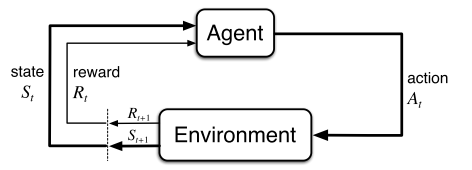
\includegraphics[width=0.7\linewidth]{chart.png}
    \caption{智能体与环境交互流程(\textbf{MDP})}
    \label{MDP_agent}
\end{figure}
\subsection{值函数与动作值函数}
在MDP框架下,给定策略$\pi$,具体而言为智能体在给定状态下选择动作的方式(可以以概率形式给出),即$p(s$状态下选择动作$a)=\pi(a|s)$。定义状态$s$的值函数如下:
$$
v_{\pi}(s) \doteq \mathbb{E}_{\pi}\left[G_{t} \mid S_{t}=s\right]=\mathbb{E}_{\pi}\left[\sum_{k=0}^{\infty} \gamma^{k} R_{t+k+1} \mid S_{t}=s\right], \text { for all } s \in \mathcal{S}
$$
表示未来的期望收益。可以写成如下的迭代形式:
$$
\begin{aligned}
v_{\pi}(s) & \doteq \mathbb{E}_{\pi}\left[G_{t} \mid S_{t}=s\right] \\
&=\mathbb{E}_{\pi}\left[R_{t+1}+\gamma G_{t+1} \mid S_{t}=s\right] \\
&=\sum_{a} \pi(a \mid s) \sum_{s^{\prime}} \sum_{r} p\left(s^{\prime}, r \mid s, a\right)\left[r+\gamma \mathbb{E}_{\pi}\left[G_{t+1} \mid S_{t+1}=s^{\prime}\right]\right] \\
&=\sum_{a} \pi(a \mid s) \sum_{s^{\prime}, r} p\left(s^{\prime}, r \mid s, a\right)\left[r+\gamma v_{\pi}\left(s^{\prime}\right)\right], \quad \text { for all } s \in \mathcal{S}
\end{aligned}
$$
上式即为\textbf{贝尔曼方程}。

下图为在均匀随机策略下的$\textbf{Grid\ World}$案例。在此例中,除移动至左上角或右下角的$\textbf{Reward}$为0外,其他状态之下的动作$\textbf{Reward}$均为-1。
\begin{figure}[hbt]
    \centering
    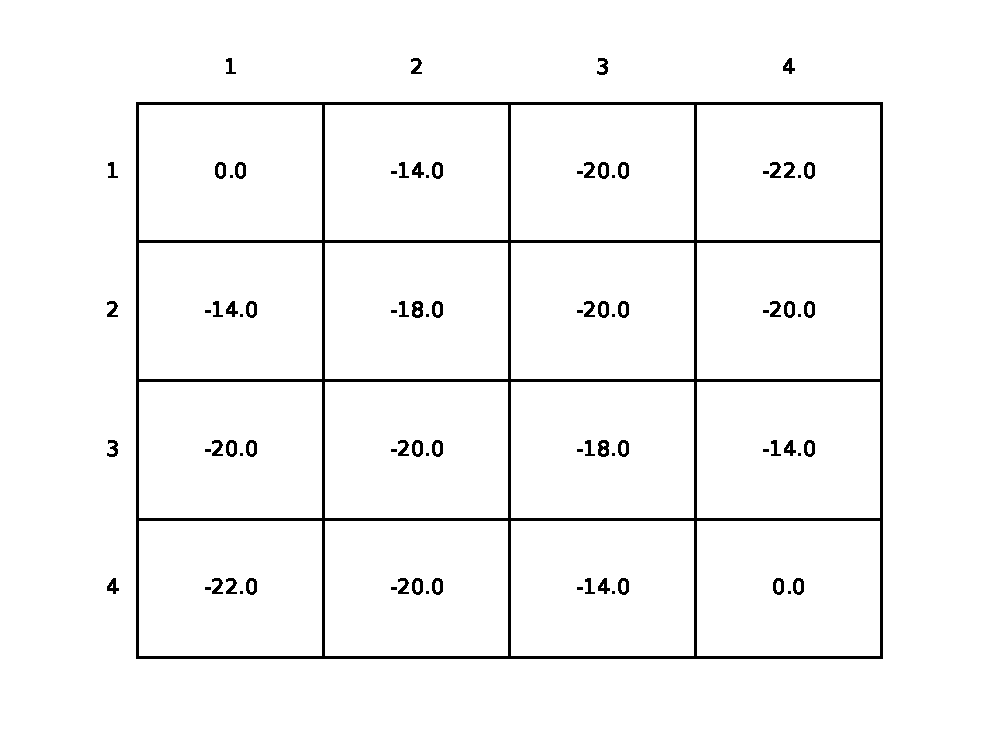
\includegraphics[width=0.6\linewidth]{gridworld.eps}
	\vspace{-0.5cm}
    \caption{Grid\ World中均匀随机策略下的值函数}
    \label{GridWorld_solution}
\end{figure}

同样可以定义状态$s$和动作$a$下的动作值函数:
$$
q_{\pi}(s, a) \doteq \mathbb{E}_{\pi}\left[G_{t} \mid S_{t}=s, A_{t}=a\right]=\mathbb{E}_{\pi}\left[\sum_{k=0}^{\infty} \gamma^{k} R_{t+k+1} \mid S_{t}=s, A_{t}=a\right]
$$
\subsection{最优策略和最优值函数}
强化学习的目标是求解问题的最优策略,即每一次动作的选择都遵循未来期望奖励最大的原则。从值函数的角度来看,就是求解最大值函数对应的策略$\pi$。即最优值函数:
$$
v_{*}(s) \doteq \max _{\pi} v_{\pi}(s)
$$
对所有 $s \in \mathcal{S}$.

相应的可以定义最优动作值函数:
$$
q_{*}(s, a) \doteq \max _{\pi} q_{\pi}(s, a)
$$
对所有 $s \in \mathcal{S}$ 和 $a \in \mathcal{A}(s)$。

做如下推导将值函数和动作值函数连接起来:
$$
q_{*}(s, a)\doteq \mathbb{E}_{*}\left[R_{t+1}+\gamma G_{t+1} \mid S_{t}=s, A_{t}=a\right]=\mathbb{E}\left[R_{t+1}+\gamma v_{*}\left(S_{t+1}\right) \mid S_{t}=s, A_{t}=a\right]
$$

再用上式推导\textbf{值函数的贝尔曼最优方程}。因为最优值函数需要选取接下来使得未来期望奖励最大的动作。即:
$$
\begin{aligned}
v_{*}(s) &=\max _{a \in \mathcal{A}(s)} q_{\pi_{*}}(s, a) \\
&=\max _{a} \mathbb{E}_{\pi_{*}}\left[G_{t} \mid S_{t}=s, A_{t}=a\right] \\
&=\max _{a} \mathbb{E}_{\pi_{*}}\left[R_{t+1}+\gamma G_{t+1} \mid S_{t}=s, A_{t}=a\right] \\
&=\max _{a} \mathbb{E}\left[R_{t+1}+\gamma v_{*}\left(S_{t+1}\right) \mid S_{t}=s, A_{t}=a\right] \\
&=\max _{a} \sum_{s^{\prime}, r} p\left(s^{\prime}, r \mid s, a\right)\left[r+\gamma v_{*}\left(s^{\prime}\right)\right] .
\end{aligned}
$$

相应的有\textbf{动作值函数的贝尔曼最优方程}。
$$
\begin{aligned}
q_{*}(s, a) &=\mathbb{E}\left[R_{t+1}+\gamma \max _{a^{\prime}} q_{*}\left(S_{t+1}, a^{\prime}\right) \mid S_{t}=s, A_{t}=a\right] \\
&=\sum_{s^{\prime}, r} p\left(s^{\prime}, r \mid s, a\right)\left[r+\gamma \max _{a^{\prime}} q_{*}\left(s^{\prime}, a^{\prime}\right)\right]
\end{aligned}
$$
\section{动态规划求解最优策略和最优值函数}
接下来利用上面求得的两个贝尔曼最优方程迭代求解最优策略和最优值函数\cite{sutton2018reinforcement}。
\subsection{策略评价}
因为贝尔曼(最优)方程已经被写成迭代式的形式。所以可以用迭代的方法来求解给定策略的值函数。即
$$
\begin{aligned}
v_{k+1}(s) & \doteq \mathbb{E}_{\pi}\left[R_{t+1}+\gamma v_{k}\left(S_{t+1}\right) \mid S_{t}=s\right] \\
&=\sum_{a} \pi(a \mid s) \sum_{s^{\prime}, r} p\left(s^{\prime}, r \mid s, a\right)\left[r+\gamma v_{k}\left(s^{\prime}\right)\right]
\end{aligned}
$$

所以求解策略的值函数的迭代过程可以写成下列形式:
% Table generated by Excel2LaTeX from sheet 'Sheet1'
\begin{table}[htbp]
  \centering
    \begin{tabular}{l}
	\bottomrule
	\bottomrule
	策略评价迭代算法,即$V \approx v_{\pi}$ \\
    \midrule
	输入:$\pi$, 给定的策略 \\
    算法参数:  $\theta>0$ 迭代终止条件 \\
    初始化 $V(s)$:除了 $V($ 最终状态 $)=0$外,其他 $s \in \mathcal{S}^{+}$的值函数任取。 \\
    Loop: \\
        \quad$\Delta \leftarrow 0$ \\
        \quad Loop for each $s \in \mathcal{S}$ : \\
            \quad \quad $v \leftarrow V(s)$  \\
            \quad \quad $V(s) \leftarrow \sum_{a} \pi(a \mid s) \sum_{s^{\prime}, r} p\left(s^{\prime}, r \mid s, a\right)\left[r+\gamma V\left(s^{\prime}\right)\right]$ \\
            \quad \quad $\Delta \leftarrow \max (\Delta,|v-V(s)|)$ \\
    until $\Delta < \theta$ \\
    \bottomrule
	\bottomrule
	\end{tabular}%
  \label{algorithm1}%
\end{table}%
\subsection{策略改进}
若对于策略$\pi$和$\pi^{\prime}$来说,如果有式子$q_{\pi}\left(s, \pi^{\prime}(s)\right) \geq v_{\pi}(s)$成立,则认为后者优于前者。

证明:
$$
\begin{aligned}
v_{\pi}(s) & \leq q_{\pi}\left(s, \pi^{\prime}(s)\right) \\
&=\mathbb{E}\left[R_{t+1}+\gamma v_{\pi}\left(S_{t+1}\right) \mid S_{t}=s, A_{t}=\pi^{\prime}(s)\right] \\
&=\mathbb{E}_{\pi^{\prime}}\left[R_{t+1}+\gamma v_{\pi}\left(S_{t+1}\right) \mid S_{t}=s\right] \\
& \leq \mathbb{E}_{\pi^{\prime}}\left[R_{t+1}+\gamma q_{\pi}\left(S_{t+1}, \pi^{\prime}\left(S_{t+1}\right)\right) \mid S_{t}=s\right] \\
&=\mathbb{E}_{\pi^{\prime}}\left[R_{t+1}+\gamma \mathbb{E}_{\pi^{\prime}}\left[R_{t+2}+\gamma v_{\pi}\left(S_{t+2}\right)\right] \mid S_{t}=s\right] \\
&=\mathbb{E}_{\pi^{\prime}}\left[R_{t+1}+\gamma R_{t+2}+\gamma^{2} v_{\pi}\left(S_{t+2}\right) \mid S_{t}=s\right] \\
& \leq \mathbb{E}_{\pi^{\prime}}\left[R_{t+1}+\gamma R_{t+2}+\gamma^{2} R_{t+3}+\gamma^{3} v_{\pi}\left(S_{t+3}\right) \mid S_{t}=s\right] \\
& \vdots \\
& \leq \mathbb{E}_{\pi^{\prime}}\left[R_{t+1}+\gamma R_{t+2}+\gamma^{2} R_{t+3}+\gamma^{3} R_{t+4}+\cdots \mid S_{t}=s\right] \\
&=v_{\pi^{\prime}}(s)
\end{aligned}
$$

所以基于策略$\pi$,选择策略$\pi^{\prime}$的方式是:
$$
\begin{aligned}
\pi^{\prime}(s) & \doteq \underset{a}{\arg \max } q_{\pi}(s, a) \\
&=\underset{a}{\arg \max } \mathbb{E}\left[R_{t+1}+\gamma v_{\pi}\left(S_{t+1}\right) \mid S_{t}=s, A_{t}=a\right] \\
&=\underset{a}{\arg \max } \sum_{s^{\prime}, r} p\left(s^{\prime}, r \mid s, a\right)\left[r+\gamma v_{\pi}\left(s^{\prime}\right)\right],
\end{aligned}
$$
我们称这样选择出来的策略$\pi^{\prime}$为贪婪策略,因为它始终选择最优动作。

如果$v_{\pi}=v_{\pi^{\prime}}$那么有:
$$
\begin{aligned}
v_{\pi^{\prime}}(s) &=\max _{a} \mathbb{E}\left[R_{t+1}+\gamma v_{\pi^{\prime}}\left(S_{t+1}\right) \mid S_{t}=s, A_{t}=a\right] \\
&=\max _{a} \sum_{s^{\prime}, r} p\left(s^{\prime}, r \mid s, a\right)\left[r+\gamma v_{\pi^{\prime}}\left(s^{\prime}\right)\right] .
\end{aligned}
$$

所以$\pi$和$\pi^{\prime}$满足贝尔曼最优方程。进而两个策略相同且为最优策略。
\subsection{策略迭代}
将策略评价部分和策略改进部分连接起来,就可以得到一个完整的求解最优策略和最优值函数的算法。即动态规划算法。
\begin{table}[htbp]
  \centering
  
    \begin{tabular}{l}	 
	\bottomrule
	\bottomrule
	策略迭代算法,即$\pi \approx \pi^{*}$ \\
    \midrule
	1. Initialization \\
    \quad $V(s) \in \mathbb{R}$ and $\pi(s) \in \mathcal{A}(s)$ arbitrarily for all $s \in \mathcal{S}$ \\
    2. Policy Evaluation \\    
	Loop: \\
        \quad$\Delta \leftarrow 0$ \\
        \quad Loop for each $s \in \mathcal{S}$ : \\
            \quad \quad $v \leftarrow V(s)$  \\
            \quad \quad $V(s) \leftarrow \sum_{a} \pi(a \mid s) \sum_{s^{\prime}, r} p\left(s^{\prime}, r \mid s, a\right)\left[r+\gamma V\left(s^{\prime}\right)\right]$ \\
            \quad \quad $\Delta \leftarrow \max (\Delta,|v-V(s)|)$ \\
    until $\Delta < \theta$ \\
	3. Policy Improvement \\
	\quad $policy-stable$ $\leftarrow$ $true$ \\
	\quad For each $s \in \mathcal{S}$ : \\
	\quad \quad $old-action$ $\leftarrow \pi(s)$ \\
	\quad \quad $\pi(s) \leftarrow \arg \max _{a} \sum_{s^{\prime}, r} p\left(s^{\prime}, r \mid s, a\right)\left[r+\gamma V\left(s^{\prime}\right)\right]$ \\
	\quad \quad If $old-action$ $\neq \pi(s)$, then $policy-stable$ $\leftarrow$ $false$  \\
	\quad If $policy-stable$, then stop and return $V \approx v_{*}$ and $\pi \approx \pi_{*}$; else go to 2 \\
    \bottomrule
	\bottomrule
	\end{tabular}%
  \label{algorithm1}%
\end{table}%


上述算法即为传统的$DP$算法。虽然可以求解最优策略和最优值函数,但是由于策略评价和策略改进两个部分的运算量差别很大,可能会导致计算过程中长时间陷入第一个部分,并且对于求解最优策略来说这些计算量是无意义或者意义不大的。

对此我们也有相应的优化方法,如在策略评价部分只迭代一次来减少这一部分的计算量,尽管理论上这种方法收敛至最优解需要无限步迭代。(ps: 蒙特卡洛方法估计动作值函数是没有被严格证明的但也很常用,因为它是很显然的)。或者在迭代部分不做求和而是求最大动作对应的值函数,这种方法的理论依据是贝尔曼最优方程。由于策略是逐渐接近最优策略的(由第二部分可以保证),这样求解的值函数也会逐渐收敛至最优策略的值函数,并且减少了很多的计算量。这种方法称为值迭代方法。

上面两种方法的思想是异步动态规划的思想。其本质是减少优化过程中不必要的计算,提高其计算效率。按照这种思想可以设计和上述方法类似的其他算法来减少计算量。不论如何,按照上面的思想设计算法的方式有一个统一的模式:\textbf{ Generalized Policy Iteration(GPI)}(广义策略迭代)。

\section{Sarsa算法}
介绍完强化学习基本的理论框架并且使用经典的动态规划进行求解之后,现在来介绍强化学习和最优化的联系。仔细观察上面动态规划算法我们可以发现:如果要使用动态规划算法进行求解,就需要提前知道所有的状态空间和动作空间的转移概率和奖励,然而这在现实中是不可行的。大多数情况下我们只能知道一部分的采样值,所以只能根据这些采样值来进行计算。由此产生了Sarsa、和Q-Learning算法。

从优化的角度来看,既然强化学习的目标为寻找最优策略,且由bellman最优方程知寻找最优策略和寻找最优价值函数是等价的,所以可以仅使用采样数据由bellman方程的迭代形式设计如下迭代形式来逐步接近最优价值函数。
$$
Q\left(s_{t}, a_{t}\right) \leftarrow Q\left(s_{t}, a_{t}\right)+\alpha\left[r_{t}+\gamma Q\left(s_{t+1}, a_{t+1}\right)-Q\left(s_{t}, a_{t}\right)\right]
$$

然后我们用贪婪算法来选取在某个状态下动作价值最大的那个动作,即 $\arg \max _{a} Q(s, a)$ 。这样似乎已经形成了一个完整的强化学习算法: 用贪婪算法根据动作价值选取动作来和环境交互,再根据得到的数据用时序差分算法更新动作价值估计。

然而这个简单的算法存在两个需要进一步考虑的问题。第一,如果要用时序差分算法来准确地估计策略的状态价值函数,我们需要用极大量 的样本来进行更新。但实际上我们可以忽略这一点,直接用一些样本来评估策略,然后就可以更新策略了。我们可以这么做的原因是策略提 升可以在策略评估末完全进行的情况进行,动态规划里的价值迭代就是这样,这其实是广义策略迭代 (generalized policy iteration)的思想。第二,如果在策略提升中一直根据贪婪算法得到一个确定性策略,可能会导致某些状态动作对 $(s, a)$从不出现, 以至于无法对其动作 价值进行估计,进而无法保证策略提升后的策略比之前的好。简单常用的解决方案是不再一味使用贪婪算法,而是采用一个 $\epsilon$-贪婪策略:有 $1-\epsilon$ 的概率采用动作价值最大的那个动作,另外有 $\epsilon$ 的概率从动作空间中随机采取一个动作,其公式表示 为:
$$
\pi(a \mid s)= \begin{cases}\epsilon /|\mathcal{A}|+1-\epsilon & \text { 如果 } a=\arg \max _{a^{\prime}} Q\left(s, a^{\prime}\right) \\ \epsilon /|\mathcal{A}| & \text { 其他动作 }\end{cases}
$$

现在,我们就可以得到一个实际的基于时序差分方法的强化学习算法。这个算法被称为 Sarsa,因为它的动作价值更新用到了当前状态 $s$ 、当 前动作 $a$ 、获得的奖励 $r$ 、一个状态 $s^{\prime}$ 和下一个动作 $a^{\prime}$ ,将这些符号拼接后就得到了算法名称。Sarsa 的具体算法如下:

- 初始化 $Q(s, a)$

- for 序列 $e=1 \rightarrow E$ do:

- -得到初始状态 $s$

- -用 $\epsilon$-greedy 策略根据 $Q$ 选择当前状态 $s$ 下的动作 $a$

- -for 时间步 $t=1 \rightarrow T$ do:

- - -得到环境反贵的 $r, s^{\prime}$

- - -用 $\epsilon$-greedy 策略根据 $Q$ 选择当前状态 $s^{\prime}$ 下的动作 $a^{\prime}$

- - -$\quad Q(s, a) \leftarrow Q(s, a)+\alpha\left[r+\gamma Q\left(s^{\prime}, a^{\prime}\right)-Q(s, a)\right]$

- - -$\quad s \leftarrow s^{\prime}, a \leftarrow a^{\prime}$

- -end for

- end for

而从最优化的角度出发,这件事情就变得非常显而易见,我的目标为寻找真实的价值函数,最简单的方法就是设计公式不断朝这个方向迭代。即不断更新价值函数使价值函数接近$r+\gamma Q\left(s^{\prime}, a^{\prime}\right)$。从而得出真实的价值函数。有了真实的价值函数那么自然就可以导出最优策略。(真实与最优的关系:价值函数是用来刻画状态未来期望价值的,如果价值函数能够刻画现实中的动作状态对,即是“真实的”,那么从其上导出的贪婪策略必为最优策略)。下图为在经典控制问题“悬崖漫步”上SARSA算法的效果图:
\begin{figure}[hbt]
    \centering
    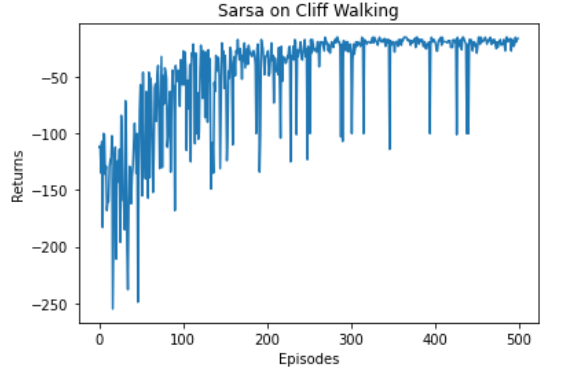
\includegraphics[width=0.6\linewidth]{SARSA.png}
	\vspace{-0.5cm}
    \caption{SARSA算法效果图(on Cliff Walking)}
    \label{SARSA}
\end{figure}

\section{Q-learning算法}
不断更新价值函数使价值函数接近$r+\gamma Q\left(s^{\prime}, a^{\prime}\right)$,目标是寻找真实的价值函数,但是SARSA算法里使用的是$\epsilon$-greedy策略,这与我们分析的“真实的价值函数的贪婪策略为最优策略”是相矛盾的。所以按照优化的思想,这里应该是按照贪婪策略取价值函数。基于这个思想的就是非常著名的基于时序差分算法的强化学习算法——Q-learning。该方法自1994年被提出\cite{rummery1994line}后,就一直被广泛使用。直到现在,这个方法及其理论仍然经久不衰。

Q-learning 和 Sarsa 的最大区别在于 Q-learning 的时 序差分更新方式为
$$
Q\left(s_{t}, a_{t}\right) \leftarrow Q\left(s_{t}, a_{t}\right)+\alpha\left[R_{t}+\gamma \max _{a} Q\left(s_{t+1}, a\right)-Q\left(s_{t}, a_{t}\right)\right]
$$

Q-learning 算法的具体流程如下:

- 初始化 $Q(s, a)$

- for 序列 $e=1 \rightarrow E$ do:

- -得到初始状态 $s$

- - for 时间步 $t=1 \rightarrow T$ do :

- - - 用 $\epsilon$-greedy 策略根据 $Q$ 选择当前状态 $s$ 下的动作 $a$

- - - 得到环境反馈的 $r, s^{\prime}$

- - - $\begin{array}{ll} & Q(s, a) \leftarrow Q(s, a)+\alpha\left[r+\gamma \max _{a^{\prime}} Q\left(s^{\prime}, a^{\prime}\right)-Q(s, a)\right] \\ & s \leftarrow s^{\prime}\end{array}$

- - end for

- end for

用优化的思想来理解 Q-learning,即 Q-learning是在直接迭代接近 $Q^{*}$ ,因为动作价值函数的贝尔曼最优方程是
$$
Q^{*}(s, a)=r(s, a)+\gamma \sum_{s^{\prime} \in \mathcal{S}} P\left(s^{\prime} \mid s, a\right) \max _{a^{\prime}} Q^{*}\left(s^{\prime}, a^{\prime}\right)
$$

怎么样,从优化的角度看,这些算法设计的动机是不是就显得非常简洁?\textbf{所以说,强化学习的算法可以看作是在特定任务情景下的优化算法}。下图为Q-learning算法在“悬崖漫步”问题上的效果图:
\begin{figure}[hbt]
    \centering
    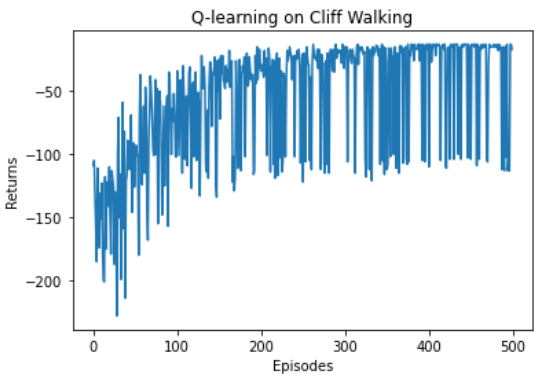
\includegraphics[width=0.6\linewidth]{Q-learning.png}
	\vspace{-0.5cm}
    \caption{Q-learning算法效果图(on Cliff Walking)}
    \label{Q-learning}
\end{figure}
\section{DQN算法}
虽然上述两种算法直接借用Bellman方程的性质巧妙地设计了优化算法,但是算法的性能较差。一方面,这是由于采样数据的不全面。另一方面是因为策略函数和值函数是非常复杂的抽象函数,直接使用这种迭代的形式进行优化很难接近其最优解。并且随着状态动作空间维数的上升,上述两种方法均不可行。

我们知道神经网络具有强大的表达能力,所以2013年有学者使用深度神经网络来近似动作值函数Q(value-base),于是强化学习算法便和优化算法更为紧密联系了起来(因为深度神经网络中最重要的一步就是基于损失函数做梯度下降\cite{王珏2006机器学习及其应用})。
\subsection{DQN算法原理}
那么 $\mathrm{Q}$ 网络的损失函数是什么呢? 回顾一下 Q-learning 的更新规则:
$$
Q(s, a) \leftarrow Q(s, a)+\alpha\left[r+\gamma \max _{a^{\prime} \in \mathcal{A}} Q\left(s^{\prime}, a^{\prime}\right)-Q(s, a)\right]
$$

上述公式用时序差分 (temporal difference,TD) 学习目标 $r+\gamma \max _{a^{\prime} \in \mathcal{A}} Q\left(s^{\prime}, a^{\prime}\right.$ ) 来增量式更新 $Q(s, a)$ ,也就是说要使 $Q(s, a)$ 和 TD 目 标 $r+\gamma \max _{a^{\prime} \in \mathcal{A}} Q\left(s^{\prime}, a^{\prime}\right)$ 靠近。于是,对于一组数据 $\left\{\left(s_{i}, a_{i}, r_{i}, s_{i}^{\prime}\right)\right\}$ ,我们可以很自然地将 Q 网络的损失函数构造为均方误差的形式:
$$
\omega^{*}=\arg \min _{\omega} \frac{1}{2 N} \sum_{i=1}^{N}\left[Q_{\omega}\left(s_{i}, a_{i}\right)-\left(r_{i}+\gamma \max _{a^{\prime}} Q_{\omega}\left(s_{i}^{\prime}, a^{\prime}\right)\right)\right]^{2}
$$

所以,一方面强化学习算法现在被归结为一类非线性最小二乘问题。另一方面将 Q-learning 扩展到神经网络形式——深度 Q 网络(deep Q network,DQN) 算法。这极大的提高了算法的可操作性,因为我们有很多方式来处理最小二乘和神经网络这两类问题。由于 DQN 是离线策略算法,因此 我们在收集数据的时候可以使用一个 $\epsilon$-贪婪策略来平衡探索与利用,将收集到的数据存储起来,在后续的训练中使用。从而帮助 DQN 取得稳定、出色的性能。下图为DQN算法在Open AI提供的gym训练环境:cartpole-v0上的效果图:
\begin{figure}[hbt]
    \centering
    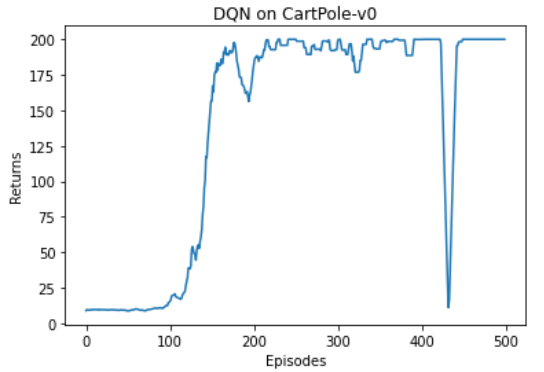
\includegraphics[width=0.6\linewidth]{DQN.png}
	\vspace{-0.5cm}
    \caption{DQN算法效果图(车杆模型)}
    \label{DQN}
\end{figure}

\section{Actor-Critic算法}
DQN用神经网络近似了价值函数,自然地可以问策略函数是否可以进行近似。在DQN之后有学者建立了策略梯度的理论(这个理论非常有趣,但它过于复杂,可以参考博客\cite{PG}),该理论直接建立了动作值函数和策略梯度的关系,于是可以使用神经网络来直接近似策略函数。所以DQN之后就有了Actor-Critic算法。
\subsection{策略梯度理论}
要求策略函数的梯度,首先需要将策略参数化。假设目标策略 $\pi_{\theta}$ 是一个随机性策略,并且处处可微,其中 $\theta$ 是对应的参数。我们可以用一个线性模 型或者神经网络模型来为这样一个策略函数建模,输入某个状态,然后输出一个动作的概率分布。我们的目标是要寻找一个最优策略并最大 化这个策略在环境中的期望回报。我们将策略学习的目标函数定义为:
$$
J(\theta)=\mathbb{E}_{s_{0}}\left[V^{\pi_{\theta}}\left(s_{0}\right)\right]
$$

其中, $s_{0}$ 表示初始状态。现在有了目标函数,我们将目标函数对策略 $\theta$ 求导,得到导数后,就可以用梯度上升方法来最大化这个目标函数, 从而得到最优策略。

定义策略 $\pi$ 下的状态访问分布,在此用 $\nu^{\pi}$ 表示。然后我们对目标函数求梯度,可以得到如下式子,更详细的推导过程在 \cite{PG}给出。
$$
\begin{aligned}
\nabla_{\theta} J(\theta) & \propto \sum_{s \in S} \nu^{\pi_{\theta}}(s) \sum_{a \in A} Q^{\pi_{\theta}}(s, a) \nabla_{\theta} \pi_{\theta}(a \mid s) \\
&=\sum_{s \in S} \nu^{\pi_{\theta}}(s) \sum_{a \in A} \pi_{\theta}(a \mid s) Q^{\pi_{\theta}}(s, a) \frac{\nabla_{\theta} \pi_{\theta}(a \mid s)}{\pi_{\theta}(a \mid s)} \\
&=\mathbb{E}_{\pi_{\theta}}\left[Q^{\pi_{\theta}}(s, a) \nabla_{\theta} \log \pi_{\theta}(a \mid s)\right]
\end{aligned}
$$

在策略梯度中,可以把梯度写成下面这个形式:
$$
g=\mathbb{E}\left[\sum_{t=0}^{\infty} \psi_{t} \nabla_{\theta} \log \pi_{\theta}\left(a_{t} \mid s_{t}\right)\right]
$$
其中 $\psi_{t}$ 可以有很多种形式:

1. $\sum_{t=0}^{\infty} \gamma^{t} r_{t^{\prime}}$ : 轨迹的总回报

2. $\sum_{t^{\prime}=t}^{\infty} \gamma^{t^{\prime}-t} r_{t^{\prime}}:$ 动作 $a_{t}$ 之后的回报

$3 . \sum_{t^{\prime}=t}^{\infty} r_{t^{\prime}}-b\left(s_{t}\right)$ : 基准线版本的改进

4. $Q^{\pi_{\theta}}\left(s_{t}, a_{t}\right)$ :动作价值函数

$5 \cdot A^{\pi_{\theta}}\left(s_{t}, a_{t}\right):$ 优势函数

$6 \cdot r_{t}+\gamma V^{\pi_{\theta}}\left(s_{t+1}\right)-V^{\pi_{\theta}}\left(s_{t}\right)$ : 时序差分残差
\subsection{Actor-Critic算法原理与优化方法}
Actor-Critic算法一方面用神经网络近似策略函数,利用上面的结果,进行梯度下降,这一部分称为Actor部分;另一方面借鉴DQN算法,用神经网络近似Q函数,这一部分称为Critic部分。这样就将问题变成了两个部分的优化问题,增强了算法稳定性,提高了策略的表达能力。Actor-Critic算法框架如下:

- 初始化策略网络参数 $\theta$ ,价值网络参数 $\omega$

- 不断进行如下循环 (每个循环是一条序列) :

- - 用当前策略 $\pi_{\theta}$ 采样轨迹 $\left\{s_{1}, a_{1}, r_{1}, s_{2}, a_{2}, r_{2} \ldots\right\}$

- - 为每一步数据计算: $\delta_{t}=r_{t}+\gamma V_{\omega}\left(s_{t+1}\right)-V_{\omega}(s)$

- - 更新价值参数 $w=w+\alpha_{\omega} \sum_{t} \delta_{t} \nabla_{\omega} V_{\omega}(s)$

- - 更新策略参数 $\theta=\theta+\alpha_{\theta} \sum_{t} \delta_{t} \nabla_{\theta} \log \pi_{\theta}(a \mid s)$

实际实验表明,将问题切分为两个优化问题来互相帮助进行学习,可以有效提高算法性能。下图为Actor-Critic算法在车杆模型上的效果图。相比与DQN算法,算法性能和稳定性提高了许多。
\begin{figure}[hbt]
    \centering
    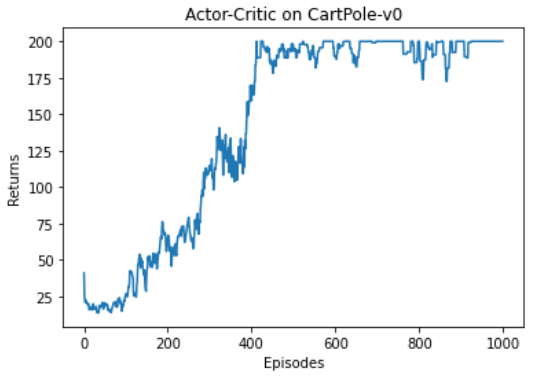
\includegraphics[width=0.6\linewidth]{Ac.png}
	\vspace{-0.5cm}
    \caption{Actor-Critic算法效果图(车杆模型)}
    \label{Actor-Critic}
\end{figure}

\section{TRPO算法}
\cite{schulman2015trust}尽管有了Actor-Critic算法,但是人们发现这个算法的效果仍然不理想,这是因为神经网络本身的不稳定性。所以人们从最优化的角度对该问题进行了重构,提出了基于共轭梯度法的强化学习算法TRPO,这使得算法的效果大大提升。
\subsection{TRPO算法原理}
Actor-Critic算法是设计衡量策略好坏的价值函数$J(\theta)$,通过梯度上升的方法来最大化这个价值函数。	但缺点是当用深度模型作为策略网络时,若步长太长,策略会突然显著变差。即方差大。所以TRPO考虑在更新时找到一块信赖域(Trust Region),在这个区域上更新策略时可以保证策略性能是上升的。这样就可以平稳地进行训练。

TRPO用下式说明了新旧策略的价值函数之间相差了一个新策略下的TD误差的期望(即等式右边第二项)。
$$\eta(\tilde{\pi})=\eta(\pi)+\sum_{s} \rho_{\tilde{\pi}}(s) \sum_{a} \tilde{\pi}(a \mid s) A_{\pi}(s, a)$$

只要保证信赖域里该期望为正值即可保证策略性能提升。
但同时这是一个NP难问题,因为新策略未知。于是TRPO作者用当前状态密度近似新策略下的状态密度。
$$
L_{\pi}(\tilde{\pi})=\eta(\pi)+\sum_{s} \rho_{\pi}(s) \sum_{a} \tilde{\pi}(a \mid s) A_{\pi}(s, a)
$$

但这又遇到了新问题,这个近似操作只有在两个分布相似度较高时才能有效(即下列不等式成立),因此要给出两个策略之间差别的刻画:KL散度\cite{schulman2015trust}。即下式:
$$
\eta(\tilde{\pi}) \leq L_{\pi}(\tilde{\pi})+C D_{\mathrm{KL}}^{\max }(\pi, \tilde{\pi}), \text { where } C\ is\ constant
$$

综上所述,可以给出一个整体的带约束优化公式,不等式约束给出了一个信赖区域,强化学习算法发展到这里,直接借鉴了约束优化理论来建立问题框架。
$$
\begin{aligned}
&\underset{\theta}{\operatorname{minimize}} L_{\theta_{\text {old }}}(\theta) \\
&\text { subject to } D_{\mathrm{KL}}^{\max }\left(\theta_{\text {old }}, \theta\right) \leq \delta .
\end{aligned}
$$

直接求解该问题比较麻烦,所以需要对问题进行一阶、二阶近似。为了求解此优化问题,TRPO接着对上式进行泰勒展开,用KKT条件得到了上述问题的解:
$$
\theta_{k+1}=\theta_{k}+\sqrt{\frac{2 \delta}{g^{T} \boldsymbol{H}^{-1} g}} \boldsymbol{H}^{-1} \boldsymbol{g}
$$
其中,$g$为梯度,$H$为约束的Hessian矩阵。

由于神经网络表示的策略函数的参数数量非常多,一般为10的三次方数量级以上,这样计算和储存Hessian矩阵非常困难。所以作者使用共轭梯度法避开了这个问题。从而设计出可行的TRPO算法。算法框架如下:

初始化策略网络参数 $\theta$ 和价值网络参数 $\omega$

- for 序列 $e=1 \rightarrow E$ do:

- - 用当前策略 $\pi_{\theta}$ 采样轨迹 $\left\{s_{1}, a_{1}, r_{1}, s_{2}, a_{2}, r_{2}, \cdots\right\}$

- - 根据收集到的数据和价值网络估计每个状态动作对的优势 $A\left(s_{t}, a_{t}\right)$

- - 计算策略目标函数的梯度 $g$

- - 用共轭梯度法计算 $\boldsymbol{x}=\boldsymbol{H}^{-1} \boldsymbol{g}$

- - 用线性搜索找到一个 $i$ 值, 并更新策略网络参数

- - $\theta_{k+1}=\theta_{k}+\alpha^{i} \sqrt{\frac{2 \delta}{\boldsymbol{x}^{T} H \boldsymbol{x}}} \boldsymbol{x}$, 其中 $i \in\{1,2, \cdots, K\}$

- - 为能提升策略并满足 $\mathrm{KL}$ 距离限制的最小整数

- - 更新价值网络参数 (与 Actor-Critic 中的更新方法相同 )

- end for

其中共轭梯度法计算 $\boldsymbol{x}=\boldsymbol{H}^{-1} \boldsymbol{g}$框架如下:

- 初始化 $r_{0}=g-H x, \quad p_{0}=r_{0}, \quad x_{0}=0$

- for $k=0 \rightarrow N$ do:

- - $\alpha_{k}=\frac{\boldsymbol{r}_{k}^{T} \boldsymbol{r}_{k}}{\boldsymbol{p}_{k}^{T} H \boldsymbol{p}_{k}} $

- - $\boldsymbol{x}_{k+1}=\boldsymbol{x}_{k}+\alpha_{k} \boldsymbol{p}_{k}$

- - $\boldsymbol{r}_{k+1}=\boldsymbol{r}_{k}-\alpha_{k} H_{p_{k}}$

- - 如果 $\boldsymbol{r}_{k+1}^{T} \boldsymbol{r}_{k+1}$ 非常小,则退出循环

- - $\beta_{k}=\frac{\boldsymbol{r}_{k+1}^{T} r_{k+1}}{r_{k}^{T} r_{k}}$

- - $\boldsymbol{p}_{k+1}=\boldsymbol{r}_{k+1}+\beta_{k} \boldsymbol{p}_{k}$

- end for

- 输出 $\boldsymbol{x}_{N+1}$

实验表明,借助共轭梯度法建立的TRPO算法效果远优于前面几种直接进行梯度下降的算法。
\begin{figure}[hbt]
    \centering
    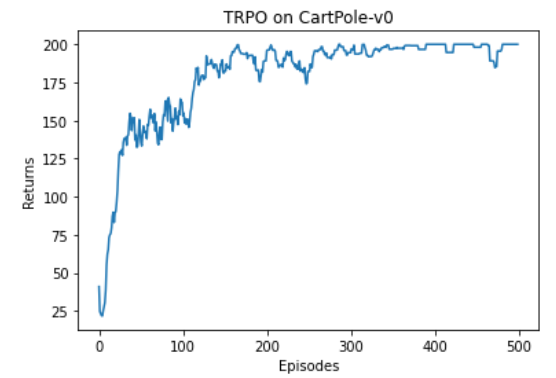
\includegraphics[width=0.6\linewidth]{TRPO.png}
	\vspace{-0.5cm}
    \caption{TRPO算法效果图(车杆模型)}
    \label{TRPO}
\end{figure}



\section{PPO算法}
虽然TRPO用共轭梯度法避开了Hessian矩阵的直接计算和储存,但是算法每次更新的计算量仍然很大。所以TRPO的作者两年后提出了PPO算法用两种方式克服了这个问题。由于TRPO的优化问题为不等式约束问题,所以人们将问题转化为罚函数的方法建立了PPO算法,它的效果更佳,打败了当时所以的强化学习算法。这使得PPO算法称为了强化学习领域近五年来最炙手可热的算法。这再一次地说明了善用最优化带来好处是无穷无尽的。

在前面优化算法的基础之上,PPO做出的改变非常简单,把TRPO里的优化问题写为重要性采样的形式,然后用两种方式避开了Hessian矩阵的求解。
$$\begin{aligned}
\underset{\theta}{\operatorname{maximize}}& \quad \hat{\mathbb{E}}_{t}\left[\frac{\pi_{\theta}\left(a_{t} \mid s_{t}\right)}{\pi_{\theta_{\text {old }}}\left(a_{t} \mid s_{t}\right)} \hat{A}_{t}\right]\\
subject to& \hat{\mathbb{E}}_{t}\left[\mathrm{KL}\left[\pi_{\theta_{\text {old }}}\left(\cdot \mid s_{t}\right), \pi_{\theta}\left(\cdot \mid s_{t}\right)\right]\right] \leq \delta
\end{aligned}$$

方法1:自适应罚函数方法
$$
L^{K L P E N}(\theta)=\hat{\mathbb{E}}_{t}\left[\frac{\pi_{\theta}\left(a_{t} \mid s_{t}\right)}{\pi_{\theta_{\text {old }}}\left(a_{t} \mid s_{t}\right)} \hat{A}_{t}-\beta \operatorname{KL}\left[\pi_{\theta_{\text {old }}}\left(\cdot \mid s_{t}\right), \pi_{\theta}\left(\cdot \mid s_{t}\right)\right]\right]
$$

- 计算 $d=\hat{\mathbb{E}}_{t}\left[\operatorname{KL}\left[\pi_{\theta_{\text {old }}}\left(\cdot \mid s_{t}\right), \pi_{\theta}\left(\cdot \mid s_{t}\right)\right]\right]$

- If $d<d_{\operatorname{targ}} / 1.5, \beta \leftarrow \beta / 2$

$-$ If $d>d_{\text {targ }} \times 1.5, \beta \leftarrow \beta \times 2$

方法2:截断法, 即把大的重要比直接截断掉。这种方法更为直接。
$$
L^{C P I}(\theta)=\hat{\mathbb{E}}_{t}\left[\frac{\pi_{\theta}\left(a_{t} \mid s_{t}\right)}{\pi_{\theta_{\text {old }}}\left(a_{t} \mid s_{t}\right)} \hat{A}_{t}\right]=\hat{\mathbb{E}}_{t}\left[r_{t}(\theta) \hat{A}_{t}\right]
$$
$$
L^{C L I P}(\theta)=\hat{\mathbb{E}}_{t}\left[\min \left(r_{t}(\theta) \hat{A}_{t}, \operatorname{clip}\left(r_{t}(\theta), 1-\epsilon, 1+\epsilon\right) \hat{A}_{t}\right)\right]
$$

虽然这两种方法非常的简单,但是效果却非常的好,这说明这两个操作对于TRPO中表述的优化问题的近似程度更高。算法收敛速度更快,稳定性更好,下面是PPO在车杆环境的效果图:
\begin{figure}[hbt]
    \centering
    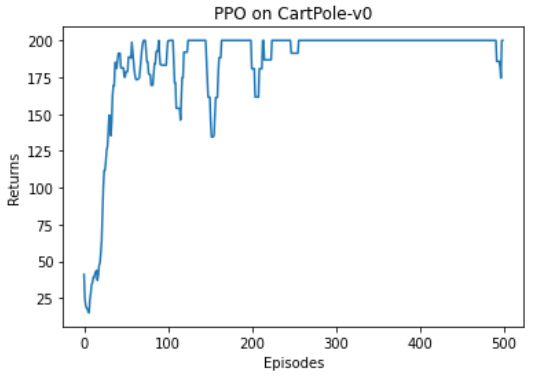
\includegraphics[width=0.6\linewidth]{PPO.png}
	\vspace{-0.5cm}
    \caption{PPO算法效果图(车杆模型)}
    \label{PPO}
\end{figure}

\section{小结}
至此,我们介绍了强化学习的理论框架:马氏决策过程(MDP\cite{sutton2018reinforcement}),介绍了动态规划\cite{geramifard2013tutorial}\cite{szepesvari1996generalized}算法,介绍了SARSA\cite{jaakkola1993convergence}和Q-learning\cite{rummery1994line}\cite{melo2001convergence}算法和最优化的联系,介绍了DQN\cite{mnih2013playing}\cite{mnih2015human}算法以及与最优化理论的联系。介绍了如何用共轭梯度法设计强化学习算法(TRPO算法\cite{schulman2015trust}),以及如何进行简化从而进一步提高算法性能(PPO算法\cite{schulman2017proximal})。在整个强化学习的算法发展历史上,优化的思想贯穿始终,发挥了至关重要的作用。所以说,\textbf{强化学习的算法可以看作是在特定任务情景下的优化算法。}由此,最优化理论对强化学习的重要性可见一斑。
\chapter{基于HMM模型的非线性共轭梯度法}
这一部分要介绍优化算法在预测任务情景下的应用。HMM模型是预测领域一类重要的模型\cite{马少辉2014客户关系动态优化模型与实证研究},通过设计转移概率公式可以很好的刻画问题情景。但是随着参数的增多,传统的极大似然估计方法不能使用,需要通过优化算法来近似求解。本研究就是使用共轭梯度法最优化一类HMM模型的参数。
\section{问题背景}
近年来直播行业非常火爆,主播在直播时通过各种才艺表演,获得关注关注、点赞、打赏。在直播情境下,随着主播对顾客施加的刺激以及刺激强度的不同,顾客在观看过程中的内在状态也会发生不同的变化。依据其所处的内在状态表现出相应的行为。

为探究直播中主播刺激对顾客内在状态和行为的影响机制,本研究建立了直播情景下顾客行为的隐状态动态优化模型,该模型将顾客在直播中的行为表现视为隐马尔可夫过程,顾客在直播中的行为是其所处隐状态的外在表现,认为顾客行为和状态的变化取决于前一时刻顾客的行为和主播在直播间中施加的刺激,并通过实际数据对模型中两类影响因素的参数进行拟合验证。
\section{HMM模型}
隐马尔科夫模型(Hidden Markov Model,以下简称HMM)是比较经典的机器学习模型,它在语言识别,自然语言处理,模式识别等领域得到广泛的应用。

对于HMM模型,首先我们假设Q是所有可能的隐藏状态的集合,V是所有可能的观测状态的集 合,即:
$$
Q=\left\{q_{1}, q_{2}, \ldots, q_{N}\right\}, V=\left\{v_{1}, v_{2}, \ldots v_{M}\right\}
$$
其中, $N$ 是可能的隐藏状态数, $M$ 是所有的可能的观察状态数。

对于一个长度为 $T$ 的序列, $I$ 对应的状态序列, $O$ 是对应的观察序列,即:
$$
I=\left\{i_{1}, i_{2}, \ldots, i_{T}\right\}, O=\left\{o_{1}, o_{2}, \ldots o_{T}\right\}
$$

HMM模型做了两个很重要的假设如下:

1) 齐次马尔科夫链假设。即任意时刻的隐藏状态只依赖于它前一个隐藏状态。当然这样假设有点 极端,因为很多时候我们的某一个隐藏状态不仅仅只依赖于前一个隐藏状态,可能是前两个或者是 前三个。但是这样假设的好处就是模型简单,便于求解。如果在时刻 $t$ 的隐藏状态是 $i_{t}=q_{i}$ , 在时刻 $t+1$ 的隐藏状态是 $i_{t+1}=q_{j}$ ,则从时刻 $t$ 到时刻 $t+1$ 的HMM状态转移概率 $a_{i j}$ 可以表示为:
$$
a_{i j}=P\left(i_{t+1}=q_{j} \mid i_{t}=q_{i}\right)
$$

这样 $a_{i j}$ 可以组成马尔科夫链的状态转移矩阵 $A$ :
$$
A=\left[a_{i j}\right]_{N \times N}
$$

2) 观测独立性假设。即任意时刻的观察状态只仅仅依赖于当前时刻的隐藏状态,这也是一个为了 简化模型的假设。如果在时刻 $t$ 的隐藏状态是 $i_{t}=q_{j}$ ,而对应的观察状态为 $o_{t}=v_{k}$ ,则 该时刻观察状态 $v_{k}$ 在隐藏状态 $q_{j}$ 下生成的概率 $b_{j}(k)$ 满足:
$$
b_{j}(k)=P\left(o_{t}=v_{k} \mid i_{t}=q_{j}\right)
$$

这样 $b_{j}(k)$ 可以组成观测状态生成的概率矩阵 $B$ :
$$
B=\left[b_{j}(k)\right]_{N \times M}
$$

除此之外,我们需要一组在时刻 $t=1$ 的隐藏状态概率分布 $\Pi$ :
$$
\Pi=[\pi(i)]_{N} \text { 其中 } \pi(i)=P\left(i_{1}=q_{i}\right)
$$

一个HMM模型,可以由隐藏状态初始概率分布 $\Pi$ ,状态转移概率矩阵 $A$ 和观测状态概率矩阵 $B$ 决定。 $\Pi, A$ 决定状态序列, $B$ 决定观测序列。因此,HMM模型可以由一个三元组 $\lambda$ 表 示如下: $\quad \lambda=(A, B, \Pi)$
\section{模型建立}
根据上述分析,我们用以下公式来表示该解析的HMM模型。
首先是给定隐状态下表现为特定的行为状态的概率公式:
$$
P(Y_{i},S_{K_1})= \frac{exp(\mu_{(s_{K_1},Y_{i})} - \beta_{(s_{K_1},Y_{i})}^{T}Y_{i})}{\Sigma_{j'=1}^{N_1}exp(\mu_{(s_{K_1},Y_{j'})} - \beta_{(s_{K_1},Y_{j'})}^{T}Y_{j'})}
$$

其次是隐状态之间的状态转移概率:
$$
P_k(S_{K_2},S_{K_1}) = \frac{exp(\gamma_{s_{(K_2,k)}} - \alpha_{s_{(K_1,k)}}^{T}W_k)}{\Sigma_{j'=1}^{N_2}exp(\gamma_{s_{(j',k)}} - \alpha_{s_{(K_1,k)}}^{T}W_k)}
$$

其中$\sigma = (\mu,\beta,\gamma,\alpha)$为模型参数。

模型的观测变量为一个三维向量:$Y_{i,t} = (X_{1,t},X_{2,t},X_{3,t})^T$。$i$为编号,$t$为时间。

将上述数据转化为这样的形式:$Y_j$ ,表示第j种行为向量。其中,
$j=1,2,...,N_1,N_1 = n_1*n_2*n_3,\quad n_1,n_2,n_3$分别为行为向量第1,2,3维度上的离散值种数。

于是,可以定义观测矩阵$B_k = (P_k(Y_{i},Y_{j}))_{N_1\times N_1}$。其中$k =1,2,...,|W|,\ W$为思维刺激向量。其转移概率公式如下:
$$\begin{aligned}
P_k(Y_{i},Y_{j}) &= \Sigma_{K_1,K_2}^{N_2} P(Y_{i},S_{K_1}) P_k(S_{K_2},S_{K_1})P(Y_{j},S_{K_2})\\
&= \Sigma_{K_1,K_2}^{N_2}\frac{exp(\mu_{(s_{K_1},Y_{i})} - \beta_{(s_{K_1},Y_{i})}^{T}Y_{i})}{\Sigma_{j'=1}^{N_1}exp(\mu_{(s_{K_1},Y_{j'})} - \beta_{(s_{K_1},Y_{j'})}^{T}Y_{j'})}\\
&* \frac{exp(\gamma_{s_{(K_2,k)}} - \alpha_{s_{(K_1,k)}}^{T}W_k)}{\Sigma_{j'=1}^{N_2}exp(\gamma_{s_{(j',k)}} - \alpha_{s_{(K_1,k)}}^{T}W_k)}\\
&*
\frac{exp(\mu_{(s_{K_2},Y_{j})} - \beta_{(s_{K_2},Y_{j})}^{T}Y_{j})}{\Sigma_{j'=1}^{N_1}exp(\mu_{(s_{K_2},Y_{j'})} - \beta_{(s_{K_2},Y_{j'})}^{T}Y_{j'})}
\end{aligned}$$

虽然上述观测状态转移式只是基于一种刺激的HMM模型,缺乏普遍性。但是它有很好的理论性质,所以可以通过全概率公式在这基础上自然导出基于多种刺激的隐马尔科夫链状态转移矩阵。令$N_1$为观测状态个数,$N_2$为隐藏状态个数。它们分别的状态转移概率公式为:
$$\begin{aligned}
P_{k_1,k_2}(Y_1,Y_3) &= \Sigma_{j=1}^{N_1}P_{k_1 }(Y_1,Y_j)P_{ k_2}(Y_j,Y_3)\\
P_{k_1,k_2}(S_1,S_3) &= \Sigma_{j=1}^{N_2}P_{k_1}(S_1,S_j)P_{k_2}(S_j,S_3)
\end{aligned}$$

上述公式为基于两个刺激${k_1,k_2}$的状态转移概率公式。同时可通过归纳法进一步给出k种刺激的状态转移公式。

然后,我们使用一种最幼稚的方式的求解上述公式的参数。首先根据数据将对应的观测转移概率估计出来,利用估计值和理论值的均方误差来设计优化算法。即下列优化问题:
$$\begin{aligned}
mi&n_{\sigma} \quad \Sigma_{k=1}^{N_3}||P_k(Y_{i},Y_{j} | \sigma) - \hat{P_k}(Y_{i},Y_{j} | \sigma)||_F^2(Frobenius \ norm)\\
&\sigma = (\mu,\beta,\gamma,\alpha),\quad k = 1,2,3,4.\\
&\mu=(\mu_{(s_i,y_j)})^T\in R^{N_1*N_2},\ \gamma=(\gamma_{(y_i,W_k)})^T \in R^{|W|* N_2},\\
&\beta=(\beta_{y_i}) \in R^{|Y|\times N_1*N_2},\beta_{y_i} = (\beta_{(s_{j},y_{k})})^T\\
&\alpha=(\alpha_{k}) \in R^{|W|\times N_2},\alpha_k = (\alpha_{(s_i,W_k)})^T
\end{aligned}$$
其中:$N_3$为刺激种类数,
$$\begin{aligned}
\hat{P_k}(Y_{t},Y_{t-1} | \sigma) = \frac{1}{n}\Sigma_{i=1}^{n}\hat{P_k}(Y_{i,t},Y_{i,t-1} | \sigma)\\
{P_k}(Y_{t},Y_{t-1} | \sigma) = \frac{1}{n}\Sigma_{i=1}^{n}{P_k}(Y_{i,t},Y_{i,t-1} | \sigma)
\end{aligned}$$

上述问题可以使用最优化相关理论和算法进行分析求解。在这里使用非线性共轭梯度法来求解这个问题。算法框架为

步1. 取初始点 $x_{0}$ 及终止参数 $\varepsilon \geq 0, d_{0}=-g_{0}$. 令 $k=0$.

步 2 . 若 $\left\|g_{k}\right\| \leq \varepsilon$, 算法终止, 否则进入下一步.

步3. 按照一定的步长规则(FR,PR,CW,Dixon规则)选取步长 $\alpha_{k 1}^{1}$ 

步4. 计算 $x_{k+1}=x_{k}+\alpha_{k} d_{k}, g_{k+1}=\nabla f\left(x_{k+1}\right)$。

核心代码为:
\begin{lstlisting}
# 非线性共轭梯度算法框架
    def nonlinear_cg(self, sigma0, Y, W, Pij, searching, beta_para):
        print('---------BEGIN---------')
        start = time.time()
        x_old = sigma0
        g_old = self.gfun(x_old, Y, W, Pij)
        # print("1:", g_old)
        d_old = -g_old
        f_list = []
        for k in range(self.kmax):
            f_old = self.fun(x_old, Y, W, Pij)
            print("当前残差函数值:", f_old)
            if k % 100 == 0:
                print(f_old)
            f_list.append(f_old[0])
            g_old_norm = np.linalg.norm(g_old, 2)
            print('当前迭代第{}步,当前精度值{:.8f}'.format(k, g_old_norm))
            if g_old_norm < self.eps:
                break
            alpha = searching(x_old, Y, W, Pij, d_old, g_old, f_old)
            # 更新 x
            x_new = x_old + alpha * d_old
            # 计算当前迭代点的梯度
            g_new = self.gfun(x_new, Y, W, Pij)
            beta = beta_para(g_old, g_new)
            d_new = -g_new + beta * d_old

            #更新参数
            d_old = d_new
            g_old = g_new
            x_old = x_new
        end = time.time()
        time_use = end - start
        return x_new, f_list, k, time_use
\end{lstlisting}
\section{问题求解}
为简化问题,实验中只选取一种刺激进行实验。实验结果如下图。代码见附录(函数和梯度函数很长)。

在模型参数拟合过程中,精确值随着迭代次数的增加首先急速下降,随后在第25次迭代后逐渐趋于平稳,并且精确值处于较小的可接受水平。该结果表明,模型参数拟合效果较好,本模型在直播情境中较为适用,模型参数值可以较为合理地描述直播过程中主播施加的刺激对顾客状态和行为表现的影响及程度。
\begin{figure}[hbt]
    \centering
    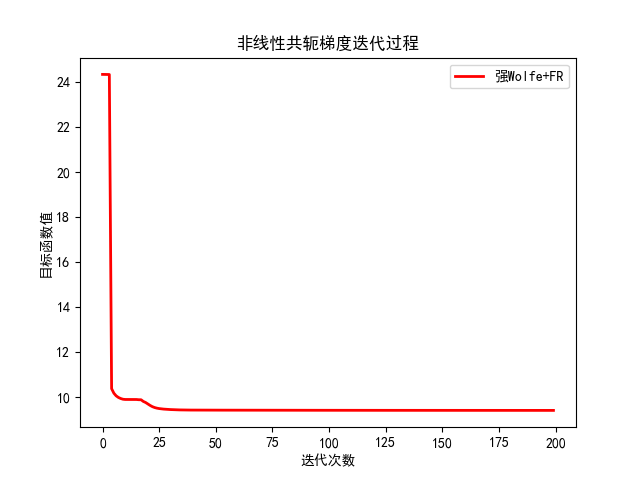
\includegraphics[width=0.6\linewidth]{非线性共轭梯度法rand.png}
	\vspace{-0.5cm}
    \caption{共轭梯度法算法效果图(车杆模型)}
    \label{gonge}
\end{figure}

本模型具有较强的实际应用价值,不仅可以动态估计直播过程中各刺激对顾客状态动态演化的影响,还可以估计顾客在直播间的外在行为所处隐状态的概率分布,从而衡量和验证顾客隐状态划分的合理性和刺激因素影响的有效性,利于研究人员和主播从业者了解直播间内的顾客特点和情况,同时主播可根据本直播间刺激因素对顾客行为的影响效果制定直播策略,有助于主播根据直播效果目标和顾客行为优化直播内容,提升直播质量,提高直播情境下顾客关系管理的效率与科学性。


\chapter{旅行商问题求解}
\section{旅行商问题}
旅行商问题(TravelingSalesmanProblem,TSP)是一个经典的组合优化问题。经典的TSP可以描述为:一个商品推销员要去若干个城市推销商品,该推销员从一个城市出发,需要经过所有城市后,回到出发地。应如何选择行进路线,以使总的行程最短。

从图论的角度来看,该问题实质是在一个带权完全无向图中,找一个权值最小的Hamilton回路。由于该问题的可行解是所有顶点的全排列,随着顶点数的增加,会产生组合爆炸,它是一个NP完全问题。由于其在交通运输、电路板线路设计以及物流配送等领域内有着广泛的应用,国内外学者对其进行了大量的研究。早期的研究者使用精确算法求解该问题,常用的方法包括:分枝定界法、线性规划法、动态规划法等。但是,随着问题规模的增大,精确算法将变得无能为力,因此,在后来的研究中,国内外学者重点使用近似算法或启发式算法,主要有遗传算法、模拟退火法、蚁群算法、禁忌搜索算法、贪婪算法和神经网络等。\cite{陈文兰2006旅行商问题算法研究综述}
\begin{figure}[hbt]
    \centering
    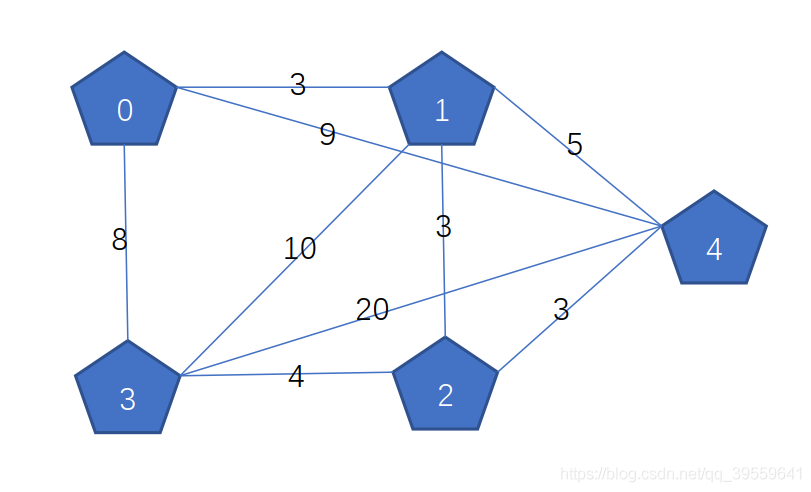
\includegraphics[width=0.6\linewidth]{旅行商.png}
	\vspace{-0.5cm}
    \caption{旅行商问题简单示例}
    \label{旅行商}
\end{figure}

TSP的研究历史很久,最早的描述是1759年欧拉研究的骑士环游问题,即对于国际象棋棋盘中的64个方格,走访64个方格一次且仅一次,并且最终返回到起始点。1954年,Geo-eDanzig等人用线性规划的方法取得了旅行商问题的历史性的突破——解决了美国49个城市的巡回问题。这就是割平面法,这种方法在整数规划问题上也广泛应用。后来还提出了一种方法叫做分枝限界法,所谓限界,就是求出问题解的上、下界,通过当前得到的限界值排除一些次优解,为最终获得最优解提示方向。每次搜索下界最小的分枝,可以减小计算量。\cite{马少平朱小燕人工智能}

最早的旅行商问题的数学规划是由Dantzig(1959)等人提出,并且是在最优化领域中进行了深入研究。许多优化方法都用它作为一个测试基准。尽管问题在计算上很困难,但已经有了大量的启发式算法和精确方法来求解数量上万的实例,并且能将误差控制在1\%内。\cite{flood1956traveling} 所以接下来我们就使用几种代表性的启发式算法来求解上述问题。

\section{启发式算法解决旅行商问题($\textbf{TSP}$)}
\subsection{启发式算法}
\cite{burkard1998well}启发式算法($Heuristic Algorithm$)可以这样定义:一个基于直观或经验构造的算法,在可接受的花费(指计算时间和空间)下给出待解决组合优化问题每一个实例的一个可行解,该可行解与最优解的偏离程度一般不能被预计。现阶段,启发式算法以仿自然体算法为主,主要有蚁群算法、模拟退火法、禁忌搜索法等。\cite{丛明煜2003现代启发式算法理论研究}

但是传统启发式算法存在一些问题:一是传统启发式算法依赖于算法的组织结构信息,通用性不高,二是容易在一些并不好的解之间陷入循环。

随着启发式算法的发展,出现了元启发式算法。元启发式算法大在传统启发式算法的思想上增加了随机搜索的思想,并且不过分依赖于算法的组织结构信息。

启发式算法中的传统启发式算法和元启发式算法都不能保证获得全局最优解,但是元启发式算法由于增加了随机搜索的思想,反复执行可能收敛到全局最优解,并且元启发式算法不过分依赖算法组织结构信息,拥有更加通用启发式策略。

分类如下:
\begin{figure}[hbt]
    \centering
    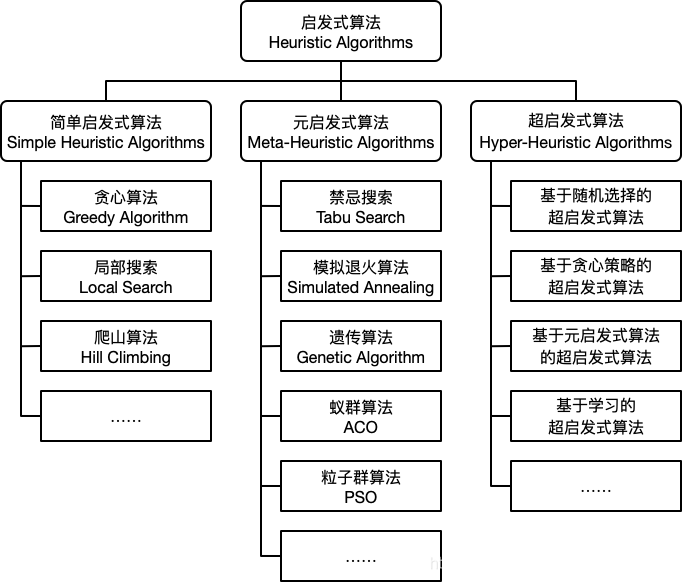
\includegraphics[width=0.8\linewidth]{启发式算法.png}
    \caption{启发式算法分类}
    \label{chart_SA}
\end{figure}

下面就四种启发式算法(模拟退火算法(SA),遗传算法(GA),蚁群算法(ACO),禁忌搜索算法(TS))简单介绍,然后使用这四种算法来求解旅行商问题。
\subsubsection{模拟退火算法(SA)}
\cite{bertsimas1993simulated}模拟退火算法思路来自于物理退火过程,在系统温度越高,退火现象指物体逐渐降温的物理现象,最终达到结晶状态,系统的能量状态最低。系统从高温降温过程中,随机选取可行解邻域内值,计算目标函数的增量值,如果系统能量下降,则接受该可行解,否则依照概率接受该解。在达到结束条件时结束循环。具体步骤如下:

$\quad \bullet$1.\ 初始化温度和终止温度,最大迭代次数,可行解

$\quad \bullet$2.\ 随机选取可行解的邻域值,计算系统能量增量,如果增量小于0则无条件接受该值;否则按照概率接受该值

$\quad \bullet$3.\ 降低温度

$\quad \bullet$4.\ 如果达到终止温度$/$最大迭代次数,则停止算法;否则跳回2

从状态1到状态2,$Metropolis$接受准则:
$$
p(1 \rightarrow 2)= \begin{cases}1 & E\left(x_{n e w}\right)<E\left(x_{\text {old }}\right) \\ \exp \left(-\frac{E\left(x_{\text {new }}\right)-E\left(x_{\text {old }}\right)}{T}\right) & E\left(x_{n e w}>=E\left(x_{\text {old }}\right)\right.\end{cases}
$$

模拟退火算法的难点在于求出产生新解的函数以及合理地调整参数提高算法的效率。
\subsubsection{遗传算法(GA)\cite{mirjalili2019genetic}}
遗传算法的思路来自于遗传与进化理论,主要包含三个阶段:自然选择,基因重组,变异。每一条染色体对应一种解决方案,首先要寻找一种从表现型到基因型的数字化编码方式,即我们需要的表现到数字化的表示过程,然后再随机初始化种群/染色体群,为了选择出适应度强的个体,我们需要构造适应度函数。随后的过程就是:选择、交叉、变异,并且为了保证种群个数不变,在选择时按照适应度高低决定被保留的概率;交叉类似于基因重组,有单点交叉、多点交叉、均匀交叉,交叉点间之间的部分依照交叉概率进行交换,最终形成新的个体;变异即是染色体任意位置编码值以一定概率反转。此算法遵循的原则与达尔文进化论的原则一致:优胜劣汰,适者生存;通过基因的交叉匹配来扩大解的区域,持续优化问题;通过基因变异添加随机扰动,避免局部最优。

步骤:

$\quad \bullet$1.\ 随机初始化种群

$\quad \bullet$2.\ 评估每条染色体的适应度

$\quad \bullet$3.\ 遵循适应度越高,被抽取概率越大的原则,从种群中选取个体作为父母本

$\quad \bullet$4.\ 父母本染色体进行交叉,产生子代

$\quad \bullet$5.\ 对自带染色体进行变异

$\quad \bullet$6.\ 在未达到循环终止条件时,跳回2

适应度函数用于评价某个个体的适应度,表现出群体中不同个体的好坏,一般总是非负的,由目标函数变换而来。选择函数用于抽取亲代中的个体,常用的选择算子有:轮盘赌选择,随即竞争选择,最佳保留选择。
\subsubsection{蚁群算法(ACO)}
1991年意大利米兰理学院M. Dorigo提出Ant System\cite{li2022circular}, 用于求解TSP等组合优化问题,这是一种模拟蚂蚁觅食行为的优化算法。

蚂蚁在运动过程中, 能够在它所经过的路径上留下外激素,而且蚂蚁在运动过程中能够感知外激素的存在及其强度,并以此指导自己的运动方向, 蚂蚁倾向于朝着外激素强度高的方向移动.由大量蚂蚁组成的蚁群的集体行为便表现出一种信息正反馈现象: 某一路径上走过的蚂蚁越多,则后来者选择该路径的概率就越大. 蚂蚁个体之间就是通过这种信息的交流达到搜索食物的目的。


蚁群算法计算过程如下:

算法原理:假如蚁群中所有蚂蚁的数量为$m$,所有城市之间的信息素用矩阵$Pheromone$表示,最短路径为$BestLength$,最佳路径为$BestTour$。每只蚂蚁都有自己的内存,内存中用一个禁忌表$Tabu$来存储该蚂蚁已经访问过的城市,表示其在以后的搜索中将不能访问这些城市;还有用另外一个允许访问的城市表$Allowed$来存储它还可以访问的城市;另外还用一个矩阵$\Delta$来存储它在一个循环(或者迭代)中给所经过的路径释放的信息素;还有另外一些数据,例如一些控制参数($\alpha,\ \beta,\ \rho,\ Q$),该蚂蚁行走玩全程的总成本或距离$TourLength$,等等。假定算法总共运行$MAX\_GEN$次,运行时间为$t$。

$\quad \bullet$1.\ 初始化。

$\quad \bullet$2.\ 为每只蚂蚁选择下一个节点。

$\quad \bullet$3.\ 更新信息素矩阵。

$\quad \bullet$4.\ 检查终止条件

$\quad \bullet$5.\ 输出最优值

如果达到最大代数$MAX\_GEN$,算法终止,转到第5步;否则,重新初始化所有的蚂蚁的$\Delta$矩阵所有元素初始化为$0$,$Tabu$表清空,$Allowed$表中加入所有的城市节点。随机选择它们的起始位置(也可以人工指定)。在$Tabu$中加入起始节点,$Allowed$中去掉该起始节点,重复执行$2,3,4$步。
\subsubsection{禁忌搜索算法(TS)}
禁忌搜索算法TS(Tabu Search)\cite{he2022hybrid}是由美国科罗拉多州大学的Fred Glover教授在1986年左右提出来的,是一个用来跳出局部最优的搜寻方法。

禁忌搜索是一种亚启发式随机搜索算法,它从一个初始可行解出发,选择一系列的特定搜索方向(移动)作为试探,选择实现让特定的目标函数值变化最多的移动。为了避免陷入局部最优解,TS搜索中采用了一种灵活的“记忆”技术,对已经进行的优化过程进行记录和选择,指导下一步的搜索方向。

TS是人工智能的一种体现,是局部领域搜索的一种扩展。禁忌搜索是在领域搜索的基础上,通过设置禁忌表来禁忌一些已经历的操作,并利用藐视准则来奖励一些优良状态,其中涉及邻域 、禁忌表、禁忌长度、候选解、藐视准则等影响禁忌搜索算法性能的关键因素。迄今为止,TS算法在组合优化等计算机领域取得了很大的成功,近年来又在函数全局优化方面得到较多的研究,并大有发展的趋势。

算法步骤如下:

$\quad \bullet$1.\ 给以禁忌表$H=\Phi$,并选定一个初始解$xnow$;

$\quad \bullet$2.\ 满足停止规则时,停止计算,输出结果;否则,在$xnow$的邻域$N(xnow)$中选择不受禁忌的候选集$Can\_N(xnow)$;在$Can\_N(xnow)$中选一个评价值最佳的解$xnext,xnow=xnext$;更新历史记录$H$,保存$f(xnow$),重复2;

$\quad \bullet$3.\ 在保存的众多$f$中,挑选最小(大)值作为解;

\subsection{实例求解}
我们使用四种算法来计算旅行商问题,分别为模拟退火算法(SA),遗传算法(GA),蚁群算法(ACO),禁忌搜索算法(TS)。
我们的问题是求解三十个城市的旅行商问题。从第一个城市出发,位置坐标以二维向量的形式给出,如$[(41,94),(37,84),(54,67),(25,62),...]$。下面是最优路径的距离关于算法迭代次数变化的可视化结果即图\ref{SAS}(代码见附录):
\begin{figure}[hbt]
    \centering
    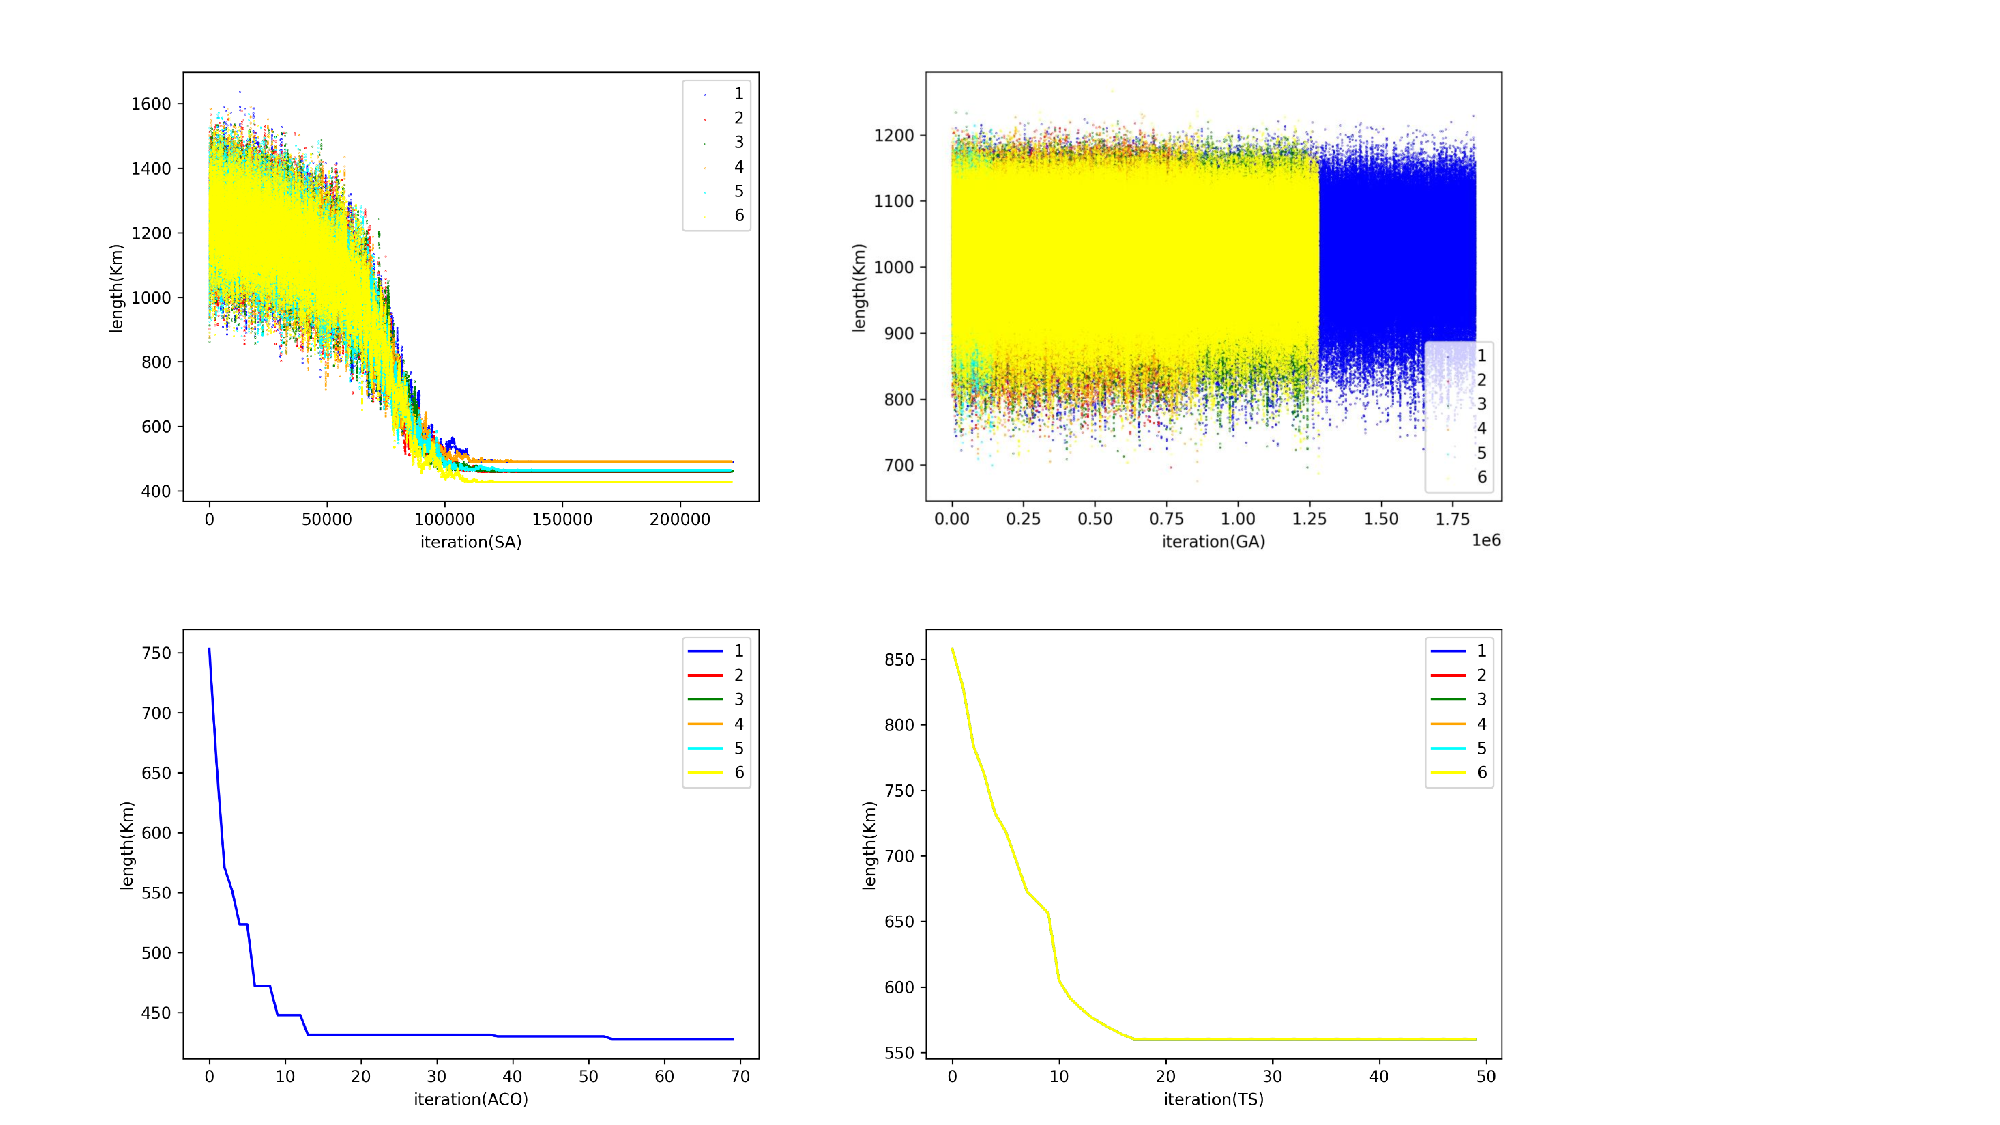
\includegraphics[width=1.2\linewidth]{SAS.pdf}
	\vspace{-0.5cm}
    \caption{距离随迭代次数下降图像}
    \label{SAS}
\end{figure}

从收敛速度上看,模拟退火算法和遗传算法在此问题中效果并不好,前者大约需要十万次迭代才能收敛;而后者完全不收敛,虽然有一些解可以达到和其他算法的解相差很少的程度,但这强烈依赖于终止条件,如果终止条件设置不好会导致算法效果大幅下降。后两种算法大幅度优于前两种算法,ACO和TS分别只需要约15次和20次即可收敛。比前两种方法快了四个数量级。

从全局最优的角度上看,SA算法和ACO算法大约可以达到$450km$的最优解。而其他两种算法分别在$700km$和$550km$左右,这说明SA和ACO算法在全局最优的角度上优于其他两种算法。

综上所述,考虑到当今时代对计算量的要求并不是很高,就算是使用Intel-i7-8750H(五年前的老版本八代CPU)版本的CPU进行计算,SA算法和ACO算法相差的时间仅为几秒(分别为5秒左右和毫秒级别);加之此问题并不需要即时的求解,对时间的要求并不高。所以我们认为用计算量换取更优的解是更值得的。因此我们将上述四种算法在旅行商问题上的性能从优到劣进行排序,分别为:$ACO>\ SA>\ TS>\ GA$。